%%%%%%%%%%%%%%%%%%%%%%%%%%%%%%%%%%%%%%%%%
% University Assignment Title Page 
% LaTeX Template
% Version 1.0 (27/12/12)
%
% This template has been downloaded from:
% http://www.LaTeXTemplates.com
%
% Original author:
% WikiBooks (http://en.wikibooks.org/wiki/LaTeX/Title_Creation)
%
% License:
% CC BY-NC-SA 3.0 (http://creativecommons.org/licenses/by-nc-sa/3.0/)
% 
% Modified for COSC480/490 by:
% Lech Szymanski (8/3/18)

\documentclass[12pt]{article}
\usepackage[draft]{cosc4x0style}
%\usepackage{cosc4x0style}

\usepackage{hyperref}
\usepackage{csquotes}
\usepackage{biblatex}
\usepackage{listings}
\usepackage{float}
\usepackage{array}
\usepackage{multirow}
\usepackage{booktabs}
\usepackage{dirtytalk}
\addbibresource{refs.bib}

% To compile the final version of the report (which will remove all the todo content)

% Specify project code 480 or 490
\papercode{480}

% Your project title
\title{An Exploration of the Common Vulnerability Scoring System}

% Your name
\author{Jake \textsc{Norton}}
\studentid{5695756}

% Names of your supervisors, separated by line break '\\'
\supervisors{
  Dr.\@ David \textsc{Eyers} \\
  Dr.\@ Veronica \textsc{Liesaputra}
}

% Date, change the \today to a set date if you want to be precise
\reportdate{\today}

\begin{document}


\maketitle

\begin{abstract}

	The Common Vulnerability Scoring System is designed to produce scores for software
	vulnerabilities. Such a system is needed in order to triage the sheer number of new
	vulnerabilities being released every year. We cannot keep up with the amount of CVSS scores that
	need to be produced, as such we need a way to automatically predict them. There is precedent to
	using machine learning, specifically in more recent times, large language models (LLMs) to
	accurately predict these CVSS scores. However, there is a general focus on only using the
	National Vulnerability Database (NVD), it would be ideal if there was more than one source for
	the ratings, not only for cross validation, but also for an increase in training data volume.
	Unfortuntately this exercise was not fruitful, and I will also continue to use NVD as the data
	source moving forward, however it is useful to look into this issue.
	Before we use any extra data sources, it will be interesting to do a comparison between the
	different sources, to see if we can get an estimated accuracy for each of the metrics within the
	scoring system. Additionally we should know how good of a system CVSS is and whether or not
	there are better alternatives. However, the ability to predict a metric based on a short text
	description is still useful, and a focus on the interpretability of such a system remains
	important.

	This paper focuses on interpretability and analysis of CVE / CVSS data, with some of the
	findings used to aid prediction of CVSS scores by LLMS.

	I will be focusing on interpretability from the data perspective. When clustering the
	data we see that there are some useful patterns
	\todo[inline]{Just some place holder for when figure out what we are doing with the clustering
		stuff}

\end{abstract}


\section{Introduction}


Last year there were 29,065 new vulnerabilities as show by Figure~\ref{fig:cve_year}. This is a
number that is only going up year on year. These vulnerabilities are recorded using the Common
Vulnerabilities and Exposure system (CVE~\cite{CVE}). From these CVEs, CVSS scores can be computed.
The National Vulnerability Database (NVD~\cite{NVD}, more on the databases in
Section~\ref{NVD_SECTION}) takes CVEs and enriches them with CVSS data. They are not the only place
to do so, however in terms of research they are often the main or sole data provider (E.g.\@
\cite{costa, nvd_example1, nvd_example2}).  I explored other options, and landed on the MITRE
database~\cite{MITRE}(details here Section~\ref{MITRE_SECTION}, as it is the main database for CVEs,
with a decent number enriched with CVSS scores. As a guideline to my investigation between the two
databases, I used the same method as the paper \textit{Can the Common Vulnerability Scoring System
	be Trusted? A Bayesian Analysis}~\cite{bayes}. This paper explores the extent to which different
data sources agree on the scoring of a CVE, aiming to gain insight into the potential for
establishing a ground truth value. Unfortunately, since that paper was released back in 2016, many
of the data sources they compared are either unavailable or in archival status. However, I hoped following
their method would still allow for insight between the two chosen databases, NVD and MITRE. This analysis
shows that the databases do fundamentally rate CVEs differently (see Figure~\ref{fig:counts}). The
uncertainty between the two can therefore be an indicator going forward when analysing generated CVE
scores, as it is likely that the model will also struggle in similar places to where the human
evaluators did. The initial focus of the work on this paper was around the CVSS and the surrounding
systems, some of the pitfalls behind the system are mentioned in the background, however while
interesting and damning in some sense, they do not stop progress towards the automation of CVSS
metric classification. Analysis between MITRE and NVD shows that it is not a system which can be
consistently rated by different evaluators / evaluation teams. Using a combination of the two
datasets is not something I will continue with going forward as the difference between the different
ratings results in confusion during training of the model.

The focus for the remainder of the paper is looking into NVD and via clustering and other dataset
analysis techniques finding patterns within the data. This will show a multitude of things, it will
show us the difference in what the models learn to treat as important versus more purely data driven
techiques. We get much quicker turn around for the analysis, Airey is currently also pursuing
interpretability from the models themselves, this takes ~48 hours per metric to run the tests. The
clustering techniques, such as Latent Dirichlet Allocation ( LDA ) take a fraction of the time, ~1
hour to cluster the entire corpus.

\todo[inline]{Placeholder for when I have more concrete example}
Additional insights gained are that some types of vulnerabilities
tend run together, for example cross site scripting and php and wordpress are found together as
there as many similar vulnerabilities using the same technologies.


\begin{figure}[h] \centering
	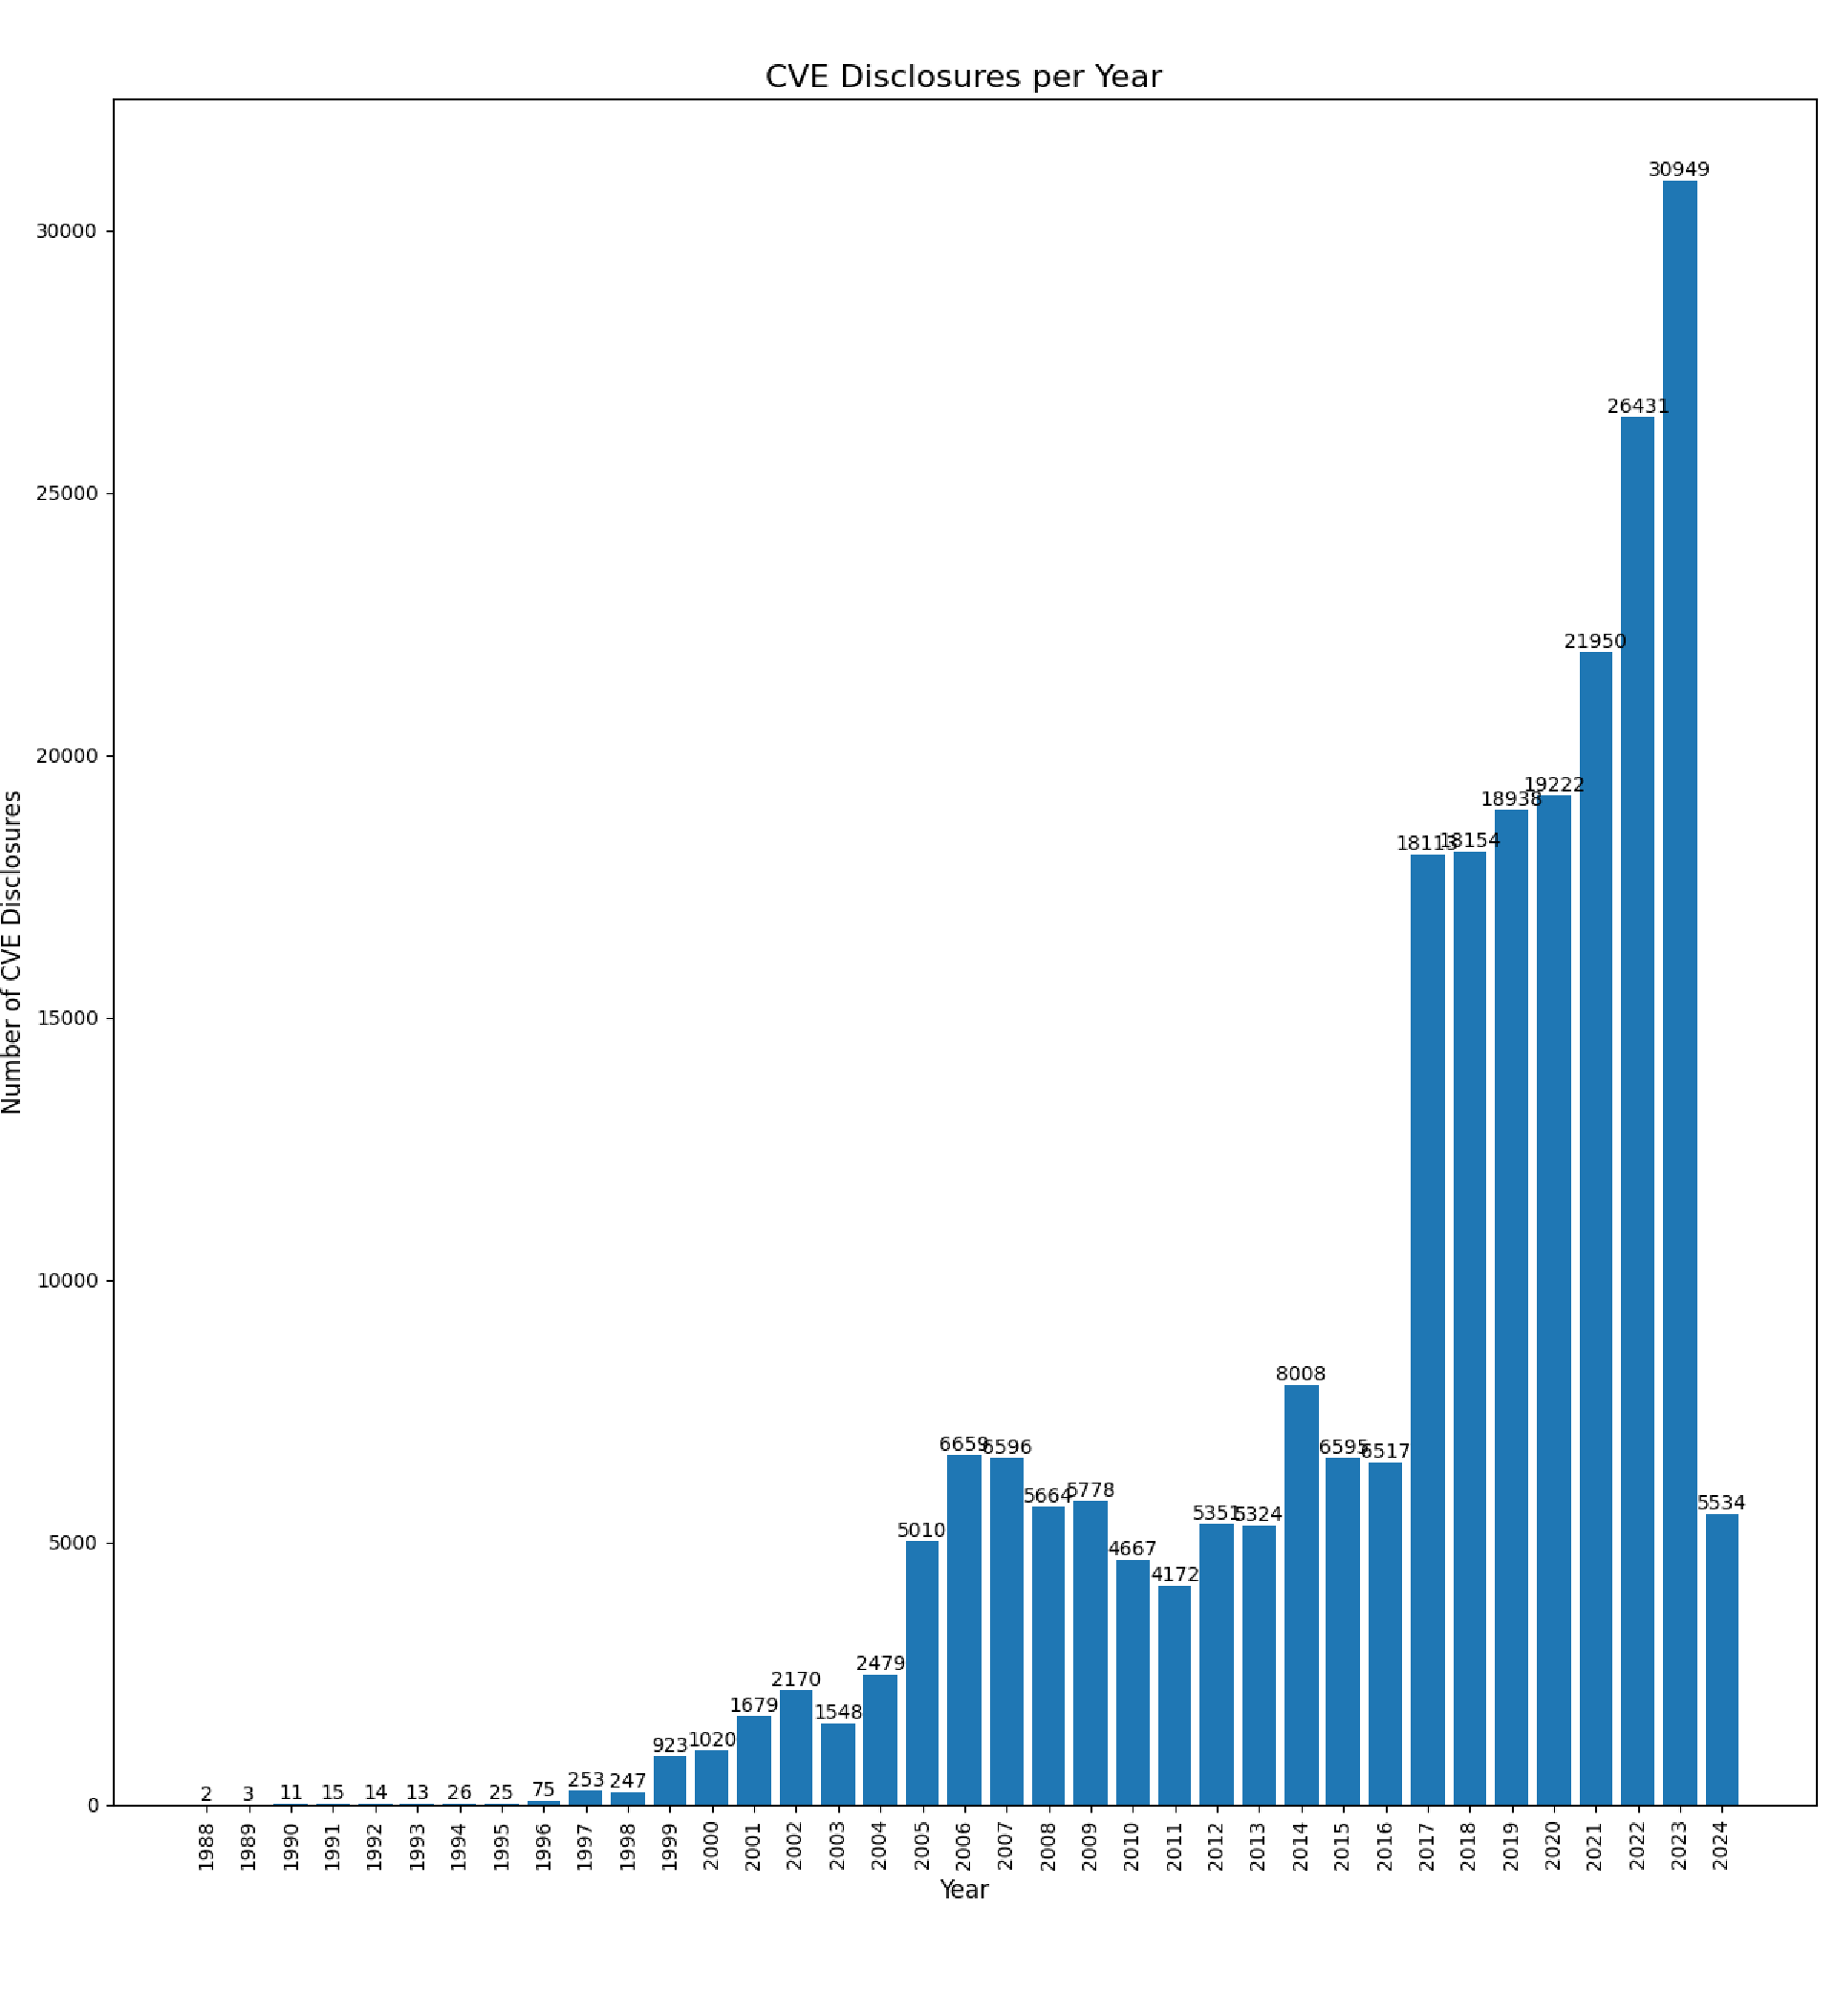
\includegraphics[width=0.8\textwidth]{figures/cves_year.pdf}
	\caption{\label{fig:cve_year}Number of new CVEs by year}
\end{figure}


\section{Background}

Vulnerabilities are stored in a consistent system called Common Vulnerabilities and
Exposures (CVE~\cite{CVE}).

\subsubsection*{Here is an example CVE}
\begin{itemize}
	\item   Unique Identifier: CVE-2024-38526
	\item   Source: GitHub, Inc.
	\item   Published:06/25/2024
	\item   Updated:06/26/2024

	\item   Description: pdoc provides API Documentation for Python Projects. Documentation
	      generated with \texttt{pdoc --math} linked to JavaScript files from polyfill.io. The polyfill.io
	      CDN has been sold and now serves malicious code. This issue has been fixed in pdoc 14.5.1.

\end{itemize}

{\footnotesize Sourced from \href{https://nvd.nist.gov/vuln/detail/CVE-2024-38526}{NVD CVE-2024-38526
	Detail} \cite{polyfill}} \\
\bigskip

This has a unique identifier, which is given by one of the CVE numbering authorities (CNA~\cite{CNA}), such as
GitHub, Google or any of these, \href{https://www.cve.org/PartnerInformation/ListofPartners}{CVE list of
	partners}~\cite{partners}.
The description is the most important part in our case. This should provide information about the
vulnerability. What can be exploited (device / software component)? How is the product affected if
the vulnerability is exploited? Ideally there would be a part of the description that relates to every metric,
unfortunately these descriptions are not necessarily suited to machine learning as the people
writing the descriptions are expecting a lot of intrinsic knowledge.

\subsection*{The Common Vulnerability Scoring System}

CVSS scoring is a high level way to break up vulnerabilities into different categories.
Organisations can use it to choose which vulnerability to focus on first. CVSS is broken up into
three distinct sections: base, temporal and environmental scores.

For brevity I will only show the specifics of CVSS 3.1~\cite{CVSS_31} as this is by far the most commonly used
version, even if it is not the most recent.

\subsubsection*{Base Score}

\begin{itemize}

	\item Attack Vector: Defines the avenues of attack that the vulnerability is open to. The more
	      open a component is, the higher the score. This can have the values: \texttt{Network},
	      \texttt{Adjacent}, \texttt{Local} and \texttt{Physical}.

	\item Attack Complexity: Describes how complex the attack is to orchestrate. Encompasses
	      questions like, what are the prerequisites? How much domain knowledge / background work is
	      necessary? How much effort does the attacker need to invest to succeed? This can have the
	      values: \texttt{Low} or \texttt{High}. \texttt{Low} gives a higher base score.

	\item Priviledges Required: The degree of privileges the user needs to complete the attack.
	      Ranging from: \texttt{None}, \texttt{Low} (e.g.\@ User level privilege), \texttt{High}
	      (e.g.\@ Administrator). The lower the privilege the higher the base score.

	\item User Interaction: Describes if the exploit requires another human user to make the attack
	      possible, E.g.\@ clicking a phishing link. This is either \texttt{None} or
	      \texttt{Required}, the score is highest when no user interaction is required.

	\item Scope: Defines if the attack can leak into other security scopes. E.g.\@~access to one
	      machine gives the ability to elevate privileges on other parts of the system. This can take
	      \texttt{Unchanged} or \texttt{Changed}, the score being highest when a scope change occurs.

	\item Confidentiality Impact: Detemines what is the impact on the information access /
	      disclosure to the attacker. This can be: \texttt{High}, \texttt{Low} or \texttt{None} with
	      \texttt{High} adding the most to the base score.

	\item Integrity Impact: Refers to the integrity of the information within the component. I.e.\@
	      could the data have been modified by the attacker. This has: \texttt{High}, \texttt{Low} or
	      \texttt{None}, as categories with \texttt{High} adding the most to the base score.

	\item Availability Impact: Refers to the impact of the attack on the availability of the
	      component. E.g.\@ the attacker taking the component off the network, denying the users
	      access. This can be: \texttt{High}, \texttt{Low} and \texttt{None} with \texttt{High} adding
	      the most to the base score.

\end{itemize}

{\footnotesize This is a summarized version of the
\href{https://www.first.org/cvss/v3.1/specification-document}{3.1 specification document
	provided by the  Forum of Incident Response and Security Teams (FIRST)}~\cite{CVSS_31}. } \\


\subsubsection*{Temporal}

\begin{itemize}

	\item Exploit Code Maturity: The state of the attack itself, e.g.\@ has this exploit been pulled
	      off in the wild or is it currently academic.

	\item Remidiation Level: Whether the exploit in question has a patch availabile.

	\item Report Confidence: The degree of confidence in the CVE report itself, the report may be in
	      early stages where not all of the information is known.

\end{itemize}

{\footnotesize This is a summarized version of the
\href{https://www.first.org/cvss/v3.1/specification-document}{3.1 specification document
	provided by the Forum of Incident Response and Security Teams (FIRST)}~\cite{CVSS_31}.}  \\
\bigskip

Temporal metrics would be useful in general for a CVSS score, however NVD do not store these
temporal metrics. As far as I can tell there is no reason given for this specifically, though
discourse
\href{https://security.stackexchange.com/questions/270257/cvss-v3-and-v3-1-missing-temporal-metrics-exploit-code-maturity-and-remediation
}{(Stack exchange post)}~\cite{stack_exchange} around the subject suggests that this is due to a lack
of verifiable reporting. From my perspective, both remidiation level and report confidence feel like
they could have scores attributed to them, however finding verifiable reports on the exploits seen
in the wild is difficult. There are two relatively new organisations on this front,
Cybersecurity \& Infrastructure Security Agency (CISA,
\href{https://www.cisa.gov/known-exploited-vulnerabilities-catalog}{public sector}) and
inthewild.org (\href{https://inthewild.io/}{private sector}~\cite{cisa}).

\subsection{Data Options}

I will be using NVD and MITRE as the sources of data. In 2016 when Johnson et al.\@ did their paper
on CVSS~\cite{bayes}, they had access to five different databases. Unfortunately only two of these
remain for modern data. There are others, but they are either in archival or proprietary status.

\subsubsection{National Vulnerability Database} \label{NVD_SECTION}

The National Vulnerability Database is the defacto standard dataset used for CVSS generation
research~\cite{costa, nvd_example1, nvd_example2}.  This makes a lot of sense as it is built
for the purpose with a team dedicated to enriching CVEs with CVSS scores. The dataset I am using was
retrieved using the NVD API in March 2024 and contains $\sim$100000 CVEs enriched with CVSS scores. This
comes in a consistently formatted JSON dump.

\subsubsection{MITRE Database}  \label{MITRE_SECTION}

MITRE is the defacto database for the storage of CVEs themselves, their database contains $\sim$40000
CVEs enriched with CVSS 3.1 scores. These are in a JSON dump retrieved in March 2024. The
format for usage is a bit more cumbersome to use. The CVSS scores are only stored as CVSS vector
strings (a simple text encoding~\cite{vector_string}). These are not hard to parse, though they are stored slightly
different between versions, as well as sometimes being inconsistent ($\sim$5000 had temporal metrics within
the vector strings in the MITRE database).

\subsubsection{Priliminary Data exploration}

The scorers for both NVD and MITRE do rate CVEs reasonably similar, one pattern you can see as shown
by Fig~\ref{fig:counts}, is that NVD generally give the most common categorical output more ratings.
They are less spread out across the full range of values. In addition, if we look at the
\texttt{Attack Complexity} metric, there is a reasonably large difference in how they are rated,
MITRE rate a lot more of the metrics with a \texttt{Low} score. This points to some of the
difficulty with this kind of rating system, while in theory there is a true value for these metrics,
it requires knowledge of the whole space around each of the vulnerabilities, this knowledge will
always vary marker to marker. The model will not have direct access to this knowledge; however, it
is hoped that it will be able to trace relationships between the different vulnerabilities and learn
this intrinsically.


\begin{figure}
	\centering
	\makebox[\textwidth][c]{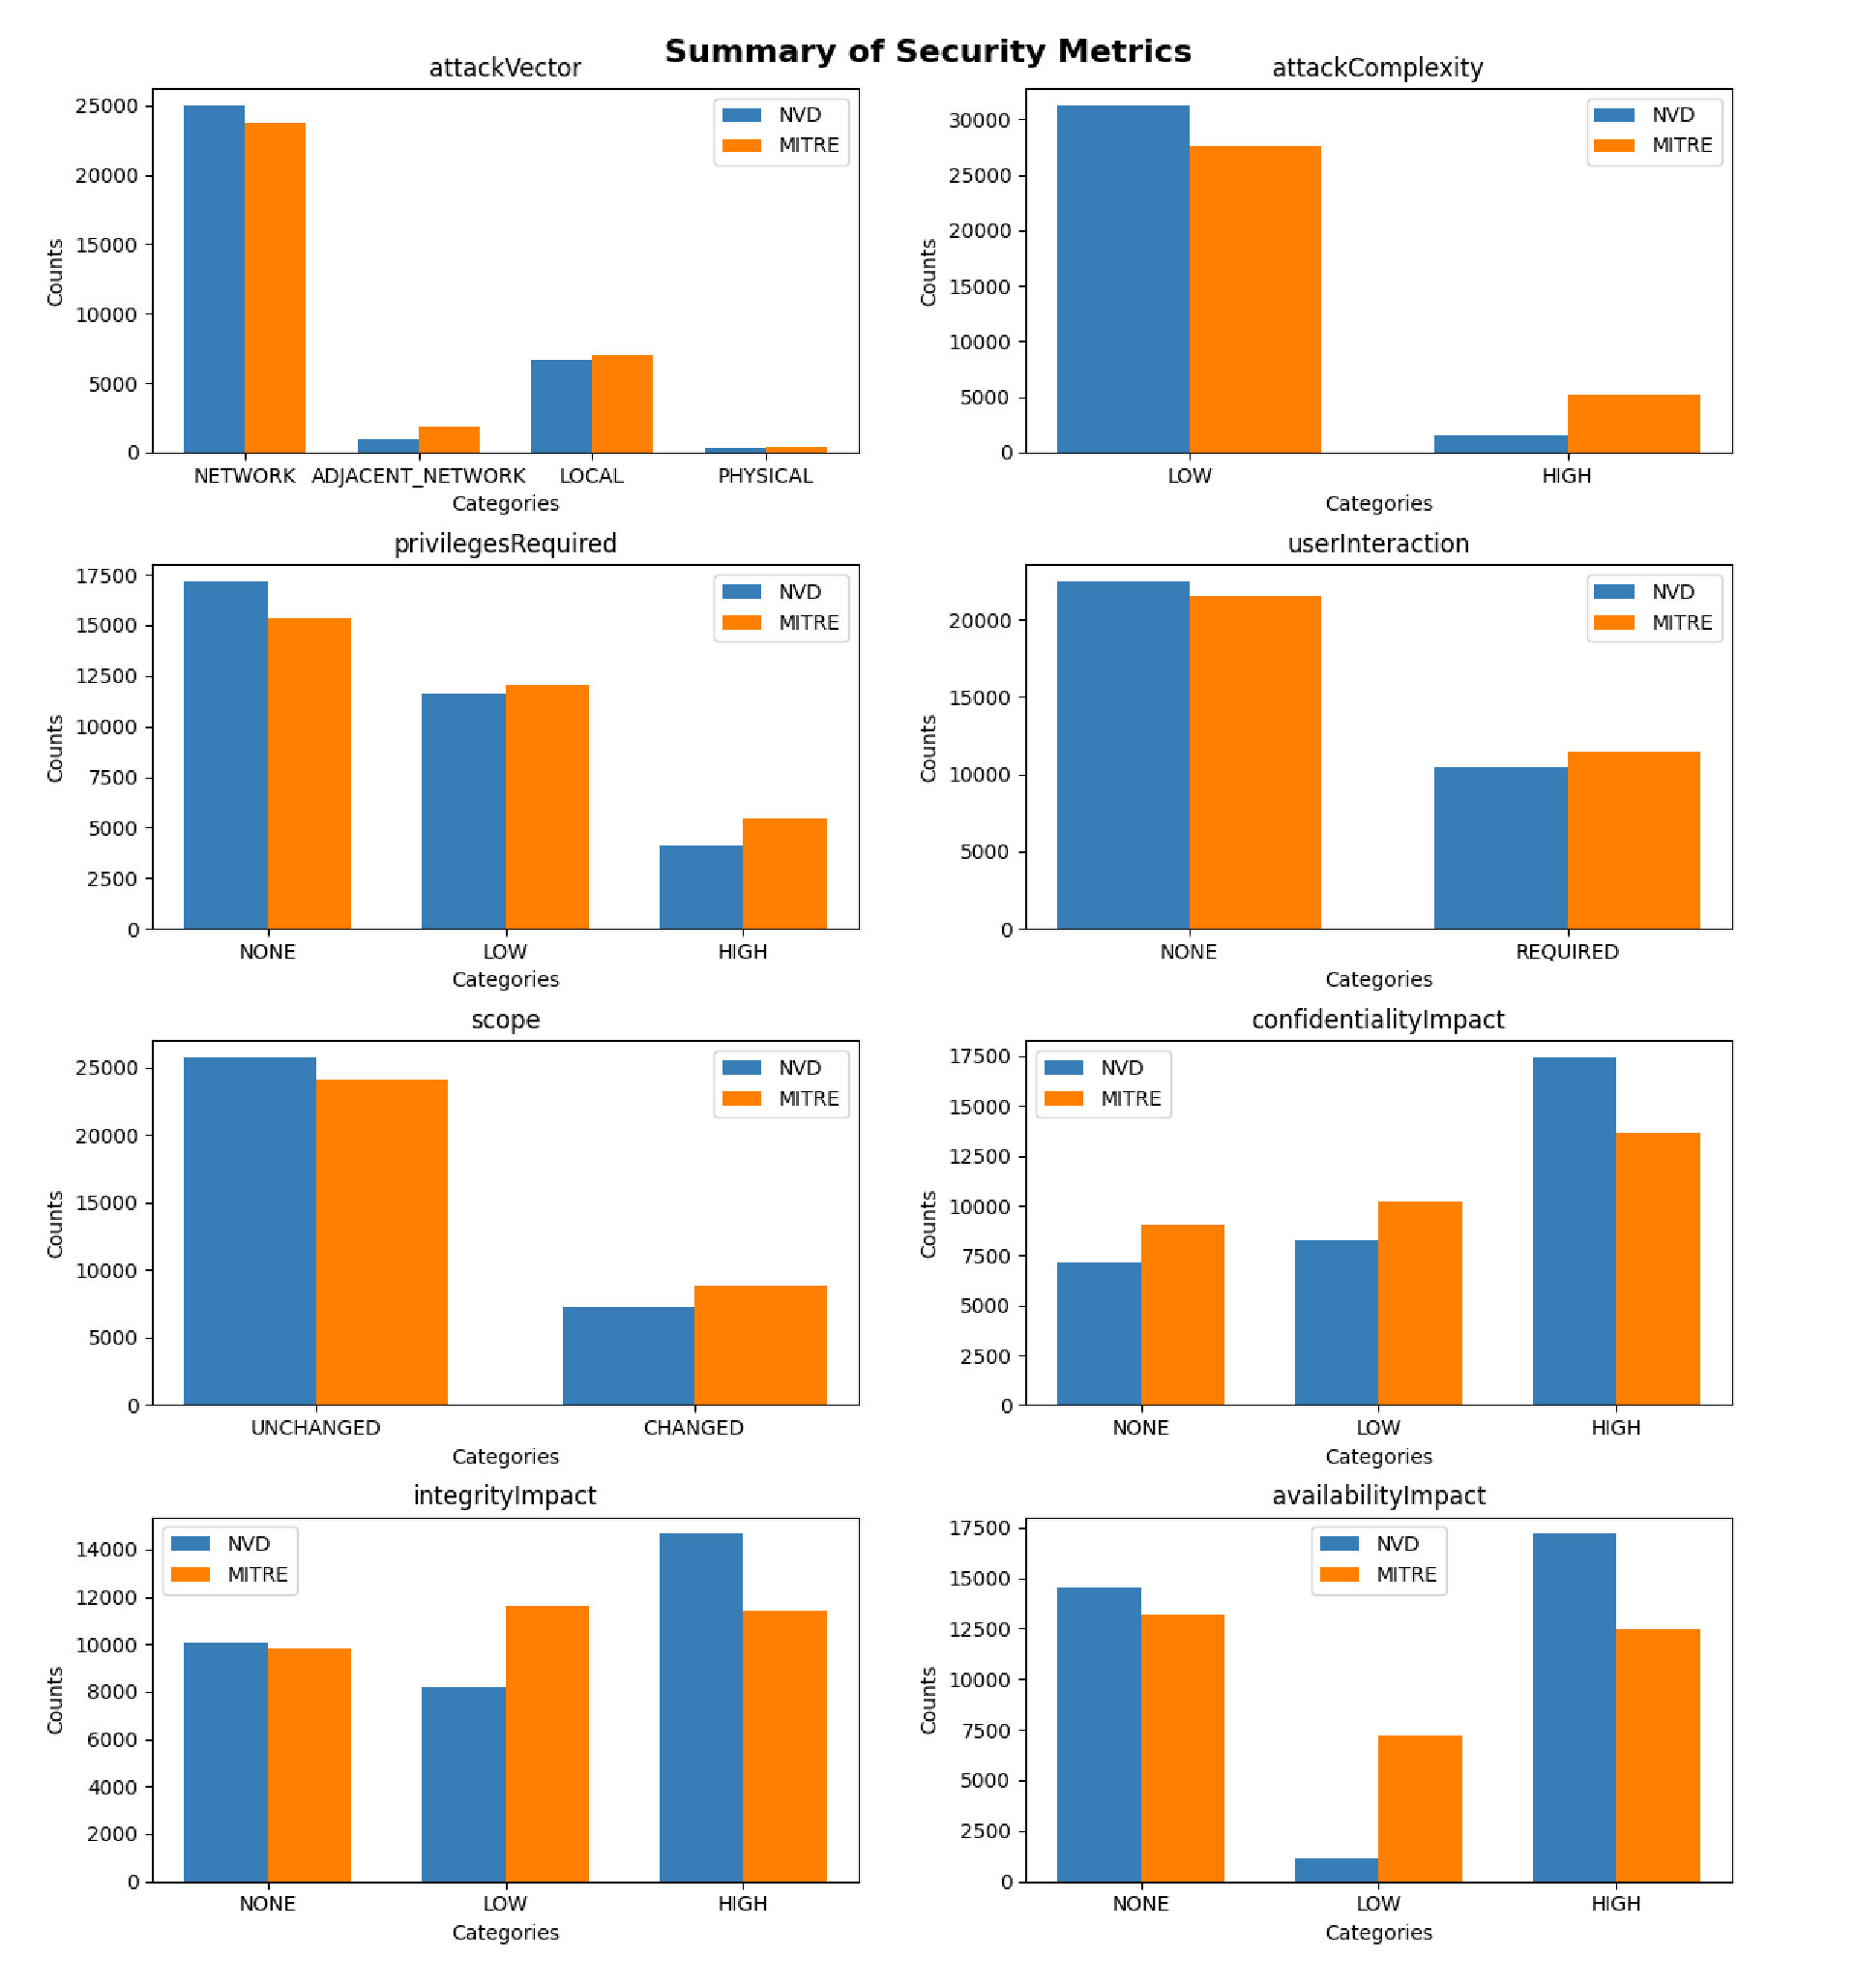
\includegraphics[width=1.2\textwidth]{figures/combined_overlap.pdf}}
	\caption{\label{fig:counts}Comparison of CVSS ratings between MITRE and NVD}
\end{figure}

\subsection{Evolution of CVSS and Its Identity Crisis}

When CVSS 2.0 was released, it was promoted as a framework to help IT management prioritize and
remediate vulnerabilities posing the greatest risk. The initial goal was to provide a comprehensive
method for assessing risk, as indicated by its original documentation:
\\

\textit{\say{Currently, IT management must identify and assess vulnerabilities across many disparate
		hardware and software platforms. They need to prioritize these vulnerabilities and remediate those
		that pose the greatest risk. But when there are so many to fix, with each being scored using
		different scales, how can IT managers convert this mountain of vulnerability data into
		actionable information? The Common Vulnerability Scoring System (CVSS) is an open framework that
		addresses this issue.}}~\cite{CVSS_2}
\\

However, by the time CVSS 3.1 was released, the framework's focus had shifted, partly due to
complaints about CVSS being a poor judge of risk. The authors stated:

\textit{\say{CVSS measures severity, not risk.}}~\cite{CVSS_31}
\\

The identity crisis is a problem because the original stance, that it can be used as a primary
prioritisation tool, has lured parts of the industry into doing just that. As mentioned by Henry
Howland in~\cite{ubiquitous}, there are many large, mainly US based places mandating the sole use of
CVSS base score for remediation. Payment Card Industry Data Security Standard~\cite{PCI}, the
Department of Defense Joint Special Access Program implementation Guide~\cite{DOD} to name a few.

This change in stance has created confusion about the true purpose of CVSS.

\subsubsection{CVSS Formula}


How CVSS is computed under-the-hood is confusing at best. CVSS 3.1 is not explained to the same
depth as version 2.0, but my understanding is that it followed a similar process. This is that
process summarised from
\href{https://www.first.org/cvss/v2/faq#Explanation-of-CVSS-v2-formula-and-metric-valued-development}{CVSS
	version 2 FAQ:}~\cite{CVSS_formula}


\begin{enumerate}
	\item  Divide the six metrics into two groups:

	      \begin{itemize}
		      \item \textbf{Impact} (3 metrics)
		      \item \textbf{Exploitability} (3 metrics)
	      \end{itemize}

	\item Create sub-vectors for each group:
	      \begin{itemize}
		      \item \textbf{Impact sub-vector}: 27 possible values ($3^3$)
		      \item \textbf{Exploitability sub-vector}: 26 possible values ($3^3 - 1$ for no impact)
	      \end{itemize}

	\item Develop and apply a series of rules to order the sub-vectors. These rules
	      are primarily based on the severity of components, e.g.\@ vectors with more
	      \texttt{Complete}
	      components are rated higher.

	\item Assign scores to the ordered sub-vectors based on the derived rules and review by the
	      Special Interest Group (SIG).

	\item Apply weightings to the sub-vectors:
	      \begin{itemize}
		      \item \textbf{Impact}: 0.6
		      \item \textbf{Exploitability}: 0.4
	      \end{itemize}

	\item \label{formula} Develop a formula that approximates the scores derived from the ordered
	      sub-vectors. Ensure the formula produces scores with $\pm$0.5 error from the originally
	      defined vector score and does not exceed the maximum value of 10.

	\item Test and refine the formula through iterations, ensuring it aligns with desired values and
	      corrects any issues, such as scores exceeding 10.

\end{enumerate}

This is process is inherently inaccurate, it is not a system designed to give precise scores. If we
look at~\ref{formula} above, the formula (\ref{equation} shows the CVSS 3.1 base score formula for
reference) which produces the score, does not match exactly the experts decision. There is a lot of
rounding and approximation going on. This is designed to make a system which is easy to use and
quick to complete by security professionals. There is a space for CVSS, however this along with the
other mentioned reasons outlines the issues with using CVSS as a sole metric for prioritization. Perhaps an option
is to triage the large swathes of new vulnerabilites coming in with an initial CVSS score, then move
on to a deeper dive. This could be in the form of the extra CVSS metrics (Temporal score \&
Environmental score), or a look into other potential options like the Exploit Prediction Scoring
System (EPSS~\cite{EPSS}).

\section{Related Work}

The main paper most similar to the Bayesian Analysis between MITRE and NVD is
\textit{Can the Common Vulnerability Scoring System be Trusted? A Bayesian
	Analysis}~\cite{bayes} by Johnson et al.\@. They conducted a study into the state of CVSS databases and their accuracy in 2016.
They found NVD to be the most correct database, and we can trust the Common~Vulnerability~Scoring~System as a
whole as scorers rate CVEs consistently. This paper will be used as the basis for the database
comparison in Section~\ref{bayesian_modeling}. This continues to be relevant in terms of process,
not so much in terms of results.

Costa et al.\@ in the paper, \textit{Predicting CVSS Metric via Description
	Interpretation}~\cite{costa}, tested generation of CVSS from CVE descriptions with a range of large
language encoder-only models. They achieved state-of-the-art results with the DistilBERT
model~\cite{distilbert}. They also improved the score with text preprocessing (e.g.\@ lemmatization)
and looked into interpretability of the models using Shapley values. This paper is relevant to
Section~\ref{cvss_prediction} as much of the process around training and inferring CVSS scores is
based on their work.

Jiang and Atif in the paper, \textit{An Approach to Discover and Assess
	Vulnerability Severity Automatically in Cyber-Physical Systems}~\cite{jiang}, create a novel
pipeline for vulnerability assessment. They used multiple data sources and a majority voting system
to decrease the chance of badly scored CVEs. This paper relates in that it shows a use case for
multiple data sources, though less so on the methods used.

Henry Howland in the paper, \textit{CVSS: Ubiquitous and Broken}~\cite{ubiquitous} broke down issues with
the CVSS system, namely, \say{lack of justification for its underlying formula, inconsistencies
	in its specification document, and no correlation to exploited vulnerabilities in the wild,
	it is unable to provide a meaningful metric for describing a vulnerability’s
	severity}~\cite{ubiquitous}.  This paper mainly relates to Section~\ref{discussion} exposing the
issues and general impression of CVSS.


\section{Methods}

\subsection{Latent Dirichlet Allocation Methodology}

Our approach to topic modeling utilizes Latent Dirichlet Allocation (LDA)~\cite{lda_origin} in conjunction with
Word2Vec~\cite{word2vec} embeddings to analyze Common Vulnerabilities and Exposures (CVE) descriptions. The
methodology comprises several key steps:

\subsubsection{Data Preprocessing} We begin by preprocessing the CVE descriptions:

\begin{itemize}

	\item Custom stopwords are defined, combining standard English stopwords with domain-specific
	      terms (e.g., "vulnerability", "attacker").

	\item Each description is tokenized and filtered, removing stopwords and short tokens (length
	      $\leq 2$).

	\item A dictionary is created from the processed texts, filtering out extremely rare and
	      extremely common terms.

\end{itemize}

\subsubsection{Word Embedding}

A Word2Vec model is trained on the preprocessed texts:

\begin{itemize} \item Vector size: 100 \item Window size: 5 \item Minimum word count: 2
\end{itemize}

This embedding captures semantic relationships between words in the CVE context.


\subsubsection{Topic Coherence Metric} We define a custom coherence metric based on Word2Vec
similarities:

\begin{equation}
	Coherence = \frac{\sum_{i=1}^{n}\sum_{j=i+1}^{n} similarity(word_i, word_j)}{\binom{n}{2}}
\end{equation}

where $n$ is the number of top words in a topic (10 in our implementation).

\subsubsection{LDA Model Training}

We employ a grid search approach to optimize LDA hyperparameters:

\begin{itemize}

	\item Number of topics: $[num\_topics, num\_topics + 1)$

	\item $\alpha$: \{"symmetric"\}

	\item $\eta$: \{0.1\}

	\item Number of passes: \{30\}

	\item Number of iterations: \{200\}

\end{itemize}

The LDA model is implemented using Gensim's LdaMulticore, allowing for parallel processing.

\subsubsection{Model Evaluation and Selection}

Models are evaluated based on the average topic coherence:

\begin{equation}
	Score = \frac{1}{T}\sum_{t=1}^{T} Coherence(topic_t)
\end{equation}

where $T$ is the total number of topics.

The top 5 models, ranked by coherence score, are saved for further analysis.

\subsubsection{Topic Assignment and Analysis}

For each saved model:

\begin{itemize}

	\item Topic assignments are generated for each document in the corpus.

	\item Results, including document index, description, assigned topic, and CVSS data, are saved
	      in JSON format.

	\item The top 50 words for each topic are extracted and saved for interpretation.

\end{itemize}

\subsection{Extended LDA Analysis on Balanced Dataset}

Following the initial LDA model training and evaluation, we perform additional steps to gain deeper insights into the relationship between topics and CVSS metrics:

\subsubsection{Balanced Dataset Analysis}

We run the LDA model on a balanced dataset to mitigate potential biases:

\begin{itemize}

	\item The dataset is balanced by undersampling or oversampling to ensure equal representation of each class within a chosen CVSS metric (e.g., Confidentiality Impact).

	\item The LDA model is then applied to this balanced dataset using the previously determined optimal parameters.

\end{itemize}

\subsubsection{Cluster-Class Association}

For each class within each CVSS metric, we identify the most representative cluster:

\begin{itemize}

	\item Calculate the proportion of documents from each class assigned to each topic cluster.

	\item Use a metric such as lift or odds ratio to determine which cluster best represents each class:

	      \begin{equation}
		      Lift(class, cluster) = \frac{P(class | cluster)}{P(class)}
	      \end{equation}

	\item The cluster with the highest lift for a given class is considered its best representative.

\end{itemize}

\subsubsection{Visualization and Interpretation}

We create visualizations to aid in the interpretation of results:

\begin{itemize}

	\item Generate heatmaps showing the distribution of classes across clusters for each CVSS metric.

	\item Create word clouds or bar charts of the most frequent terms in the representative clusters for each class.

	\item Plot multidimensional scaling (MDS) or t-SNE visualizations of document-topic distributions, colored by CVSS metric classes.

\end{itemize}

Interpretation of these visualizations involves:

\begin{itemize}

	\item Analyzing the semantic themes of representative clusters for each CVSS metric class.

	\item Identifying common vulnerability types or attack vectors associated with specific CVSS ratings.

	\item Examining any unexpected associations between topics and CVSS metrics.

\end{itemize}

\subsubsection{Cluster Merging and Refinement}

To potentially improve class representation, we explore merging related clusters:

\begin{itemize}

	\item Identify clusters with semantic similarity or overlapping representation of CVSS classes.

	\item Merge these clusters by combining their topic-word distributions and reassigning documents.

	\item Recalculate class representation metrics for the merged clusters.

	\item Compare the performance of the merged model to the original in terms of:

	      \begin{itemize}

		      \item Overall topic coherence

		      \item Clarity of class representation

		      \item Interpretability of resulting topics

	      \end{itemize}

\end{itemize}

\subsubsection{Evaluation and Insights}

Finally, we evaluate the effectiveness of our extended analysis:

\begin{itemize}

	\item Assess whether the balanced dataset analysis revealed new insights not apparent in the original model.

	\item Determine if certain CVSS metrics are more clearly represented by topic clusters than others.

	\item Evaluate the impact of cluster merging on the interpretability and usefulness of the model.

	\item Discuss potential applications of these findings in automated CVSS scoring or vulnerability triage systems.

\end{itemize}

\subsection{Hierarchical Bayesian Model} \label{bayesian_modeling}

Analysis between the NVD~\cite{NVD} and MITRE~\cite{MITRE} databases is conducted using a
hierarchical Bayesian model. This model type is particularly suitable when the population is
expected to share similarities in some respects while differing in others. In this context, while
the databases share common knowledge about vulnerabilities, they differ in the experience of the
individuals rating the metrics~\cite{bayes}.

Our model builds upon the original framework presented in Section 4.1 of~\cite{bayes}. It assumes
the existence of a true value for each CVSS dimension, acknowledging that the database sample may
deviate from this true value. These potential inaccuracies are represented using confusion matrices
(see Equation~\ref{confusion_matrix_formula}).

A key distinction from the original model is the variability in the number of categorical choices
for each CVSS metric. While the original model consistently used three variables for each CVSS
metric, our adapted model accommodates between two to four categorical choices, depending on the
specific CVSS dimension being evaluated.

\subsubsection{Confusion Matrix}

Below is an example of the confusion matrix for the CVSS dimension \texttt{Confidentiality Impact}:

\begin{equation}\label{confusion_matrix_formula}
	\Pi_{ci} = \begin{bmatrix}
		\pi_{nn} & \pi_{nl} & \pi_{nh} \\
		\pi_{ln} & \pi_{ll} & \pi_{lh} \\
		\pi_{hn} & \pi_{hl} & \pi_{hh} \\
	\end{bmatrix}
\end{equation}

where $\pi_{nn}$ denotes the probability that the database correctly assigns the score \texttt{None}
when the actual value is indeed \texttt{None}. Conversely, $\pi_{nl}$ and $\pi_{nh}$ represent
instances where \texttt{None} was not the true value, indicating an incorrect score assignment by
the database.

\subsubsection{Prior Distributions}

For categorical variables, we employ uninformative priors using Dirichlet distributions. This
approach provides a uniform prior over the probability space for all categorical options, minimizing
the influence of prior beliefs on the results. The impact of these priors is negligible for
categorical metrics with more options than the number of categories.

The confusion matrices also utilize Dirichlet distribution priors. However, we incorporate a slight
initial belief to reflect that the individuals producing scores are not acting entirely randomly and
are likely to be correct more often than not. These priors remain weak given the thousands of
observations in our dataset.

\subsubsection{Parameter Estimation}

Our parameter estimation follows the Bayesian approach, updating prior beliefs with observations to
produce posterior beliefs. We employ Markov Chain Monte Carlo (MCMC) methods, which allow for
simulating data based on the previously created distribution by sampling values that the model
believes are likely from the target distribution. This technique enables accurate sampling without
requiring all data points.

For implementation, we utilized the PyMC library~\cite{pymc}, which fulfills the same functions as
JAGS in the original paper~\cite{bayes}. PyMC facilitates the modeling process and provides robust
tools for Bayesian inference and MCMC sampling.

This methodology provides a comprehensive framework for analyzing and comparing vulnerability
scoring across different databases, accounting for the inherent uncertainties and variations in
expert assessments.

% \subsection{Hierarchical Bayesian Model} \label{bayesian_modeling}

% Analysis between the NVD~\cite{NVD} and MITRE~\cite{MITRE} databases is done with a hierarchical
% bayesian model. This type of model is suitable when you expect the population to be similar in some
% respects but different in others. In this case, they share common knowledge towards the
% vulnerability, but differ in the experience of the people rating the metrics~\cite{bayes}.  The
% model is similar to the original model (see section 4.1 of~\cite{bayes}), it assumes that there
% exists a true value for each CVSS dimension, but the database sample may not be that true value.
% These inaccuracies are represented with a confusion matrix (see
% equation~\ref{confusion_matrix_formula}). The difference from the original paper is that there is no
% longer consistently three variables for each CVSS metric, varying from two to four categorical
% choices. \\

% \bigskip

% Below is the confusion matrix of the CVSS dimension \texttt{Confidentiality Impact}


% \begin{equation}\label{confusion_matrix_formula}
% 	\Pi_ci = \begin{bmatrix}
% 		\pi_{nn} & \pi_{nl} & \pi_{nh} \\
% 		\pi_{ln} & \pi_{ll} & \pi_{lh} \\
% 		\pi_{hn} & \pi_{lh} & \pi_{hh} \\
% 	\end{bmatrix}
% \end{equation}
% \\
% where $\pi_{nn}$ denotes the probability that the current database correctly assigns the random
% vulnerability the score \texttt{None} when the actual value is the same. $\pi_{nl}$ and $\pi_{nh}$ represent
% when \texttt{None} was not the actual truth value, i.e.\@ the database produced the wrong score.

% \subsubsection{Priors}

% The priors for the categorical variables were set up with uninformative priors using a Dirichlet
% distribution. This will give a uniform prior over the probability space for all categorical options.
% This is done to not colour the outcome of the results based on prior belief, though, this prior will
% have little impact for any categorical metric which has more than the number of options for that
% metric.

% The confusion matrices also need priors, as before using Dirichlet distribution.
% However, we do want to add some initial belief to this, as the people producing scores are
% not acting completely randomly, and are likely to be right more often than not. These are still weak priors
% as the number of observations is in the thousands.

% \subsubsection{Estimation}

% This follows the Bayesian approach where to estimate the parameters: you take the prior beliefs,
% take an observation, and update these beliefs to produce posterior beliefs. In this case, the method
% involves using Markov Chain Monte Carlo methods. Broadly, this allows for simulating the data, based
% on the previously created distribution, by sampling values that the model has high belief would be
% from the target distribution. This allows for accurate sampling without having all of the data. The
% original paper used JAGS~\cite{JAGS} and R. As I am more familiar with Python I did try
% pyjags (a python wrapper around JAGS~\cite{pyjags}), however I did not find great success. Instead I used the pymc
% library~\cite{pymc} to help with the modelling. It fulfilled the same tasks that JAGS did with the
% original paper~\cite{bayes}.

\subsection{CVSS Prediction} \label{cvss_prediction}

Cody Airey --a classmate of mine-- has been working on a similar problem. He has been repoducing
results from Costa et al.\@~\cite{costa}. My choice of model for CVSS prediction will very much
bootstrap off his work. So far, a strong contender for state-of-the-art model for predicting CVSS
metrics from CVE descriptions is the DistilBERT model~\cite{distilbert}. This is a variant of
BERT~\cite{BERT}, a pre-trained deep bidirectional transformer large language model developed by
Google. DistilBERT has advantages over other BERT models in terms of performance, but also on speed
of training as well as size / memory footprint of the model.

\subsubsection{Training}

The model is trained separately for each metric. Following Airey's method, each of the eight models
were trained on five different data splits to allow for a standard deviation to be calculated, in
order to aid in reducing the chance of a \textit{lucky} data split effecting the results. The
difference between Costa et al.\@ \& Airey's work, and mine is that this model was trained on a
combination of NVD and MITRE data as opposed to just using NVD. This was converted to the same
format, a CSV containing the descriptions and the CVSS scores. This does mean there are now
$\sim$40000 duplicate CVEs and $\sim$140000 CVEs enriched with CVSS scores total.

\section{Results}

\subsection{Bayesian Analysis}

The results for the database analysis will be shown through the confusion matrices for the estimated
accuracy of both NVD and MITRE. Unfortunately it is difficult to compare my results to the original
paper~\cite{bayes} as they are on a totally different dataset. However, I will note that in general the estimated
accuracy for both datasets is much lower than the scores from the original study. Across the board NVD
often had $\sim$90\% accuracy for the highest accuracy field of any metric, with Confidentiality as
a clear outlier as seen from Table~\ref{fig:johnson_confusion_matrices}.

Some general trends are that NVD (see Figure~\ref{fig:nvd_31_confusion_matrices}) have more extreme
estimated accuracies. They do better for the higher frequency options, for the \texttt{Low} option
on \texttt{Attack Complexity} for example, NVD have 98\% estimated accuracy and 66\% for
\texttt{High} versus MITRE (see Figure~\ref{fig:mitre_31_confusion_matrices}), \texttt{Low} scored
87\% and 75\% for \texttt{High}. Instead of further analysing in this way, I will point out some of
my worries around these results, not that they are wrong per se, but that they do not really tell us
anything extra than that shown by in Figure~\ref{fig:counts}, except perhaps it is helpful to see
the results in a percentage estimated accuracy instead of a proportion. Unfortunately this is
outside of my strengths, I did some cursory exploration into if doing this sort of analysis
between two populations like this does make sense, the discourse here~\cite{stat_modeling} suggests
that such a thing can be done, though it also suggests the need for more informative priors. This
may apply in my case, and I intend on getting an expert opinion closer to home, however that will be
after this report.

Johnson et al.\@ talk about the reliability of their results saying this in section 7.1 of~\cite{bayes}:\\ \\

\textit{\say{reliability concerns
		are discussed. In this study we use five different scoring instruments - the databases. If some of
		these are generally correct, but some are generally incorrect, will not the scores of the
		incorrect ones still affect our beliefs about the actual values, thus worsening reliability? It
		turns out that this is not the case. In a simulation, two scorers were set up to be completely
		aligned, scoring 90\% complete impact in one of the CIA dimensions, while a third was unaligned
		and scoring only 10\% complete impact. Initially, all scorers are equally credible, but the
		gradual accrual of evidence impacts scorer credibility (as well as beliefs about the actual CVSS
		score distributions). Thus, as the third scorer rarely matched the other two, its credibility
		eroded, thus shrinking the weight of its advise~\cite{bayes}.}} \\

Unfortunately in my case I do not have the advantage of a potential third or more scorer. This leads
me to believe that there is a chance that incorrect scores can end up corrupting the results.

\bigskip

\begin{figure}[H]
	\centering
	\makebox[\textwidth][c]{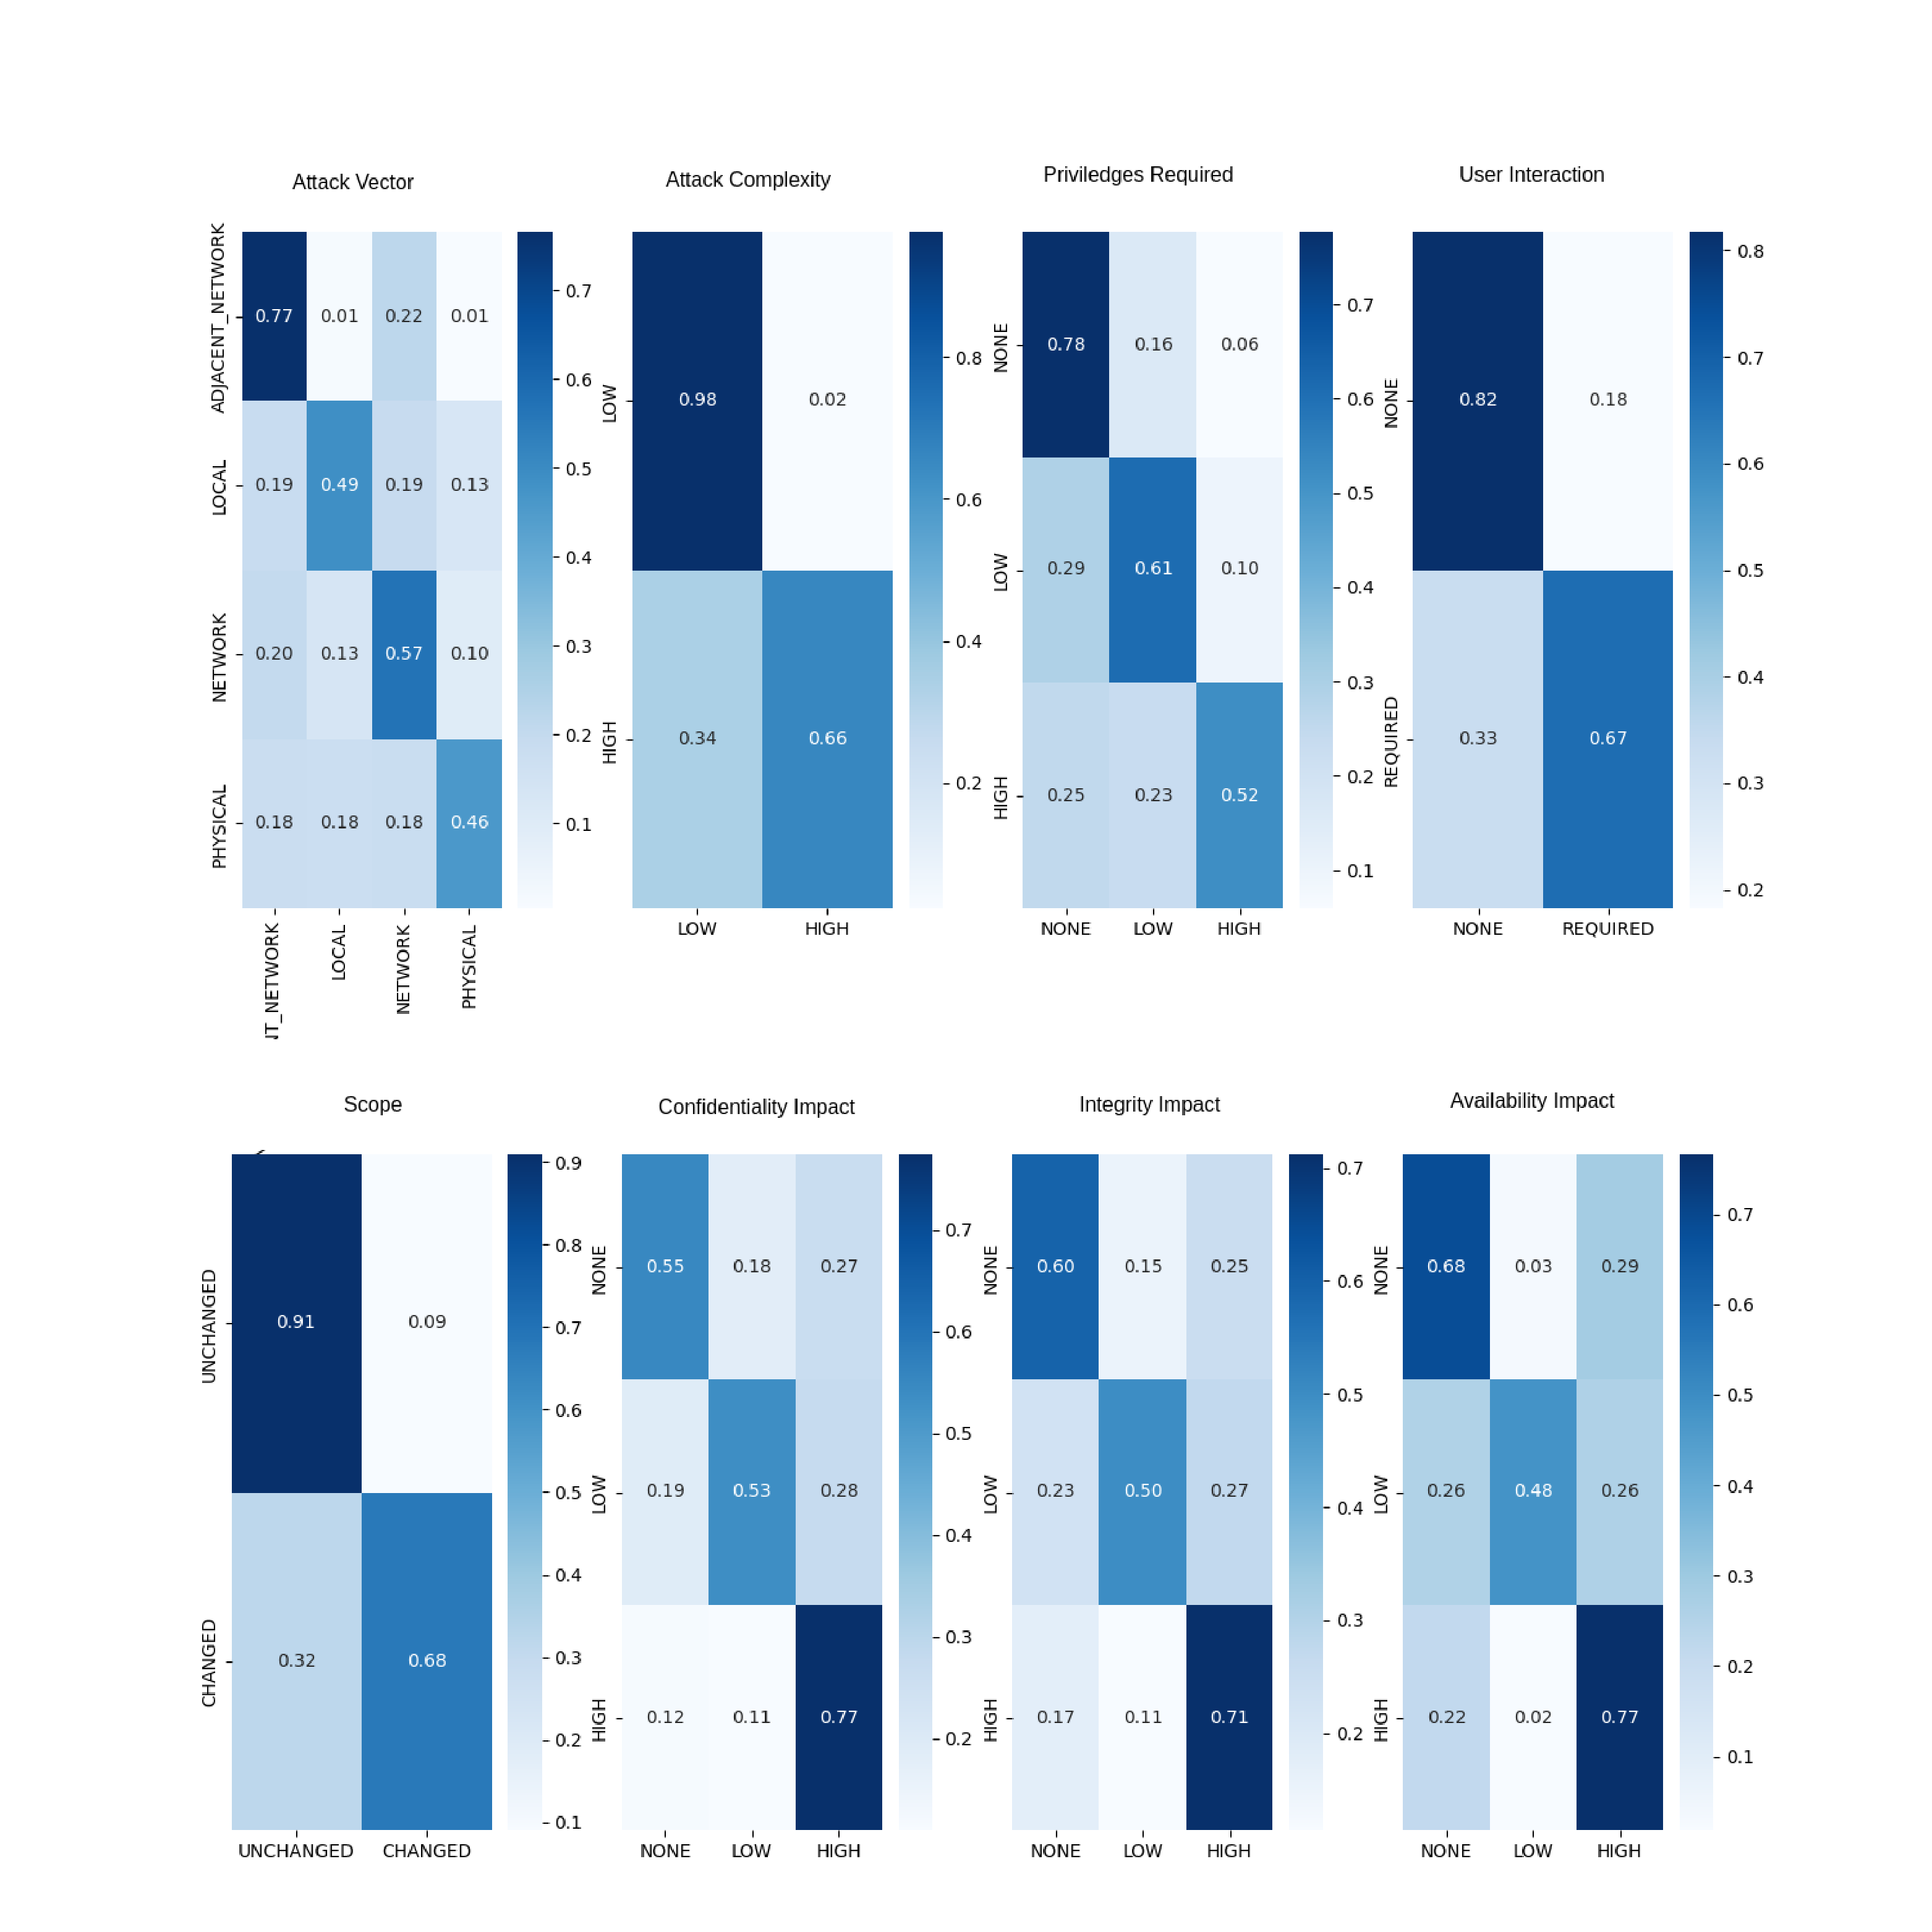
\includegraphics[width=1.5\textwidth]{figures/nvd_31_titles.pdf}}
	\caption{\label{fig:nvd_31_confusion_matrices}Confusion Matrices for NVD for CVSS version 3.1}
\end{figure}

\begin{figure}[H]
	\centering
	\makebox[\textwidth][c]{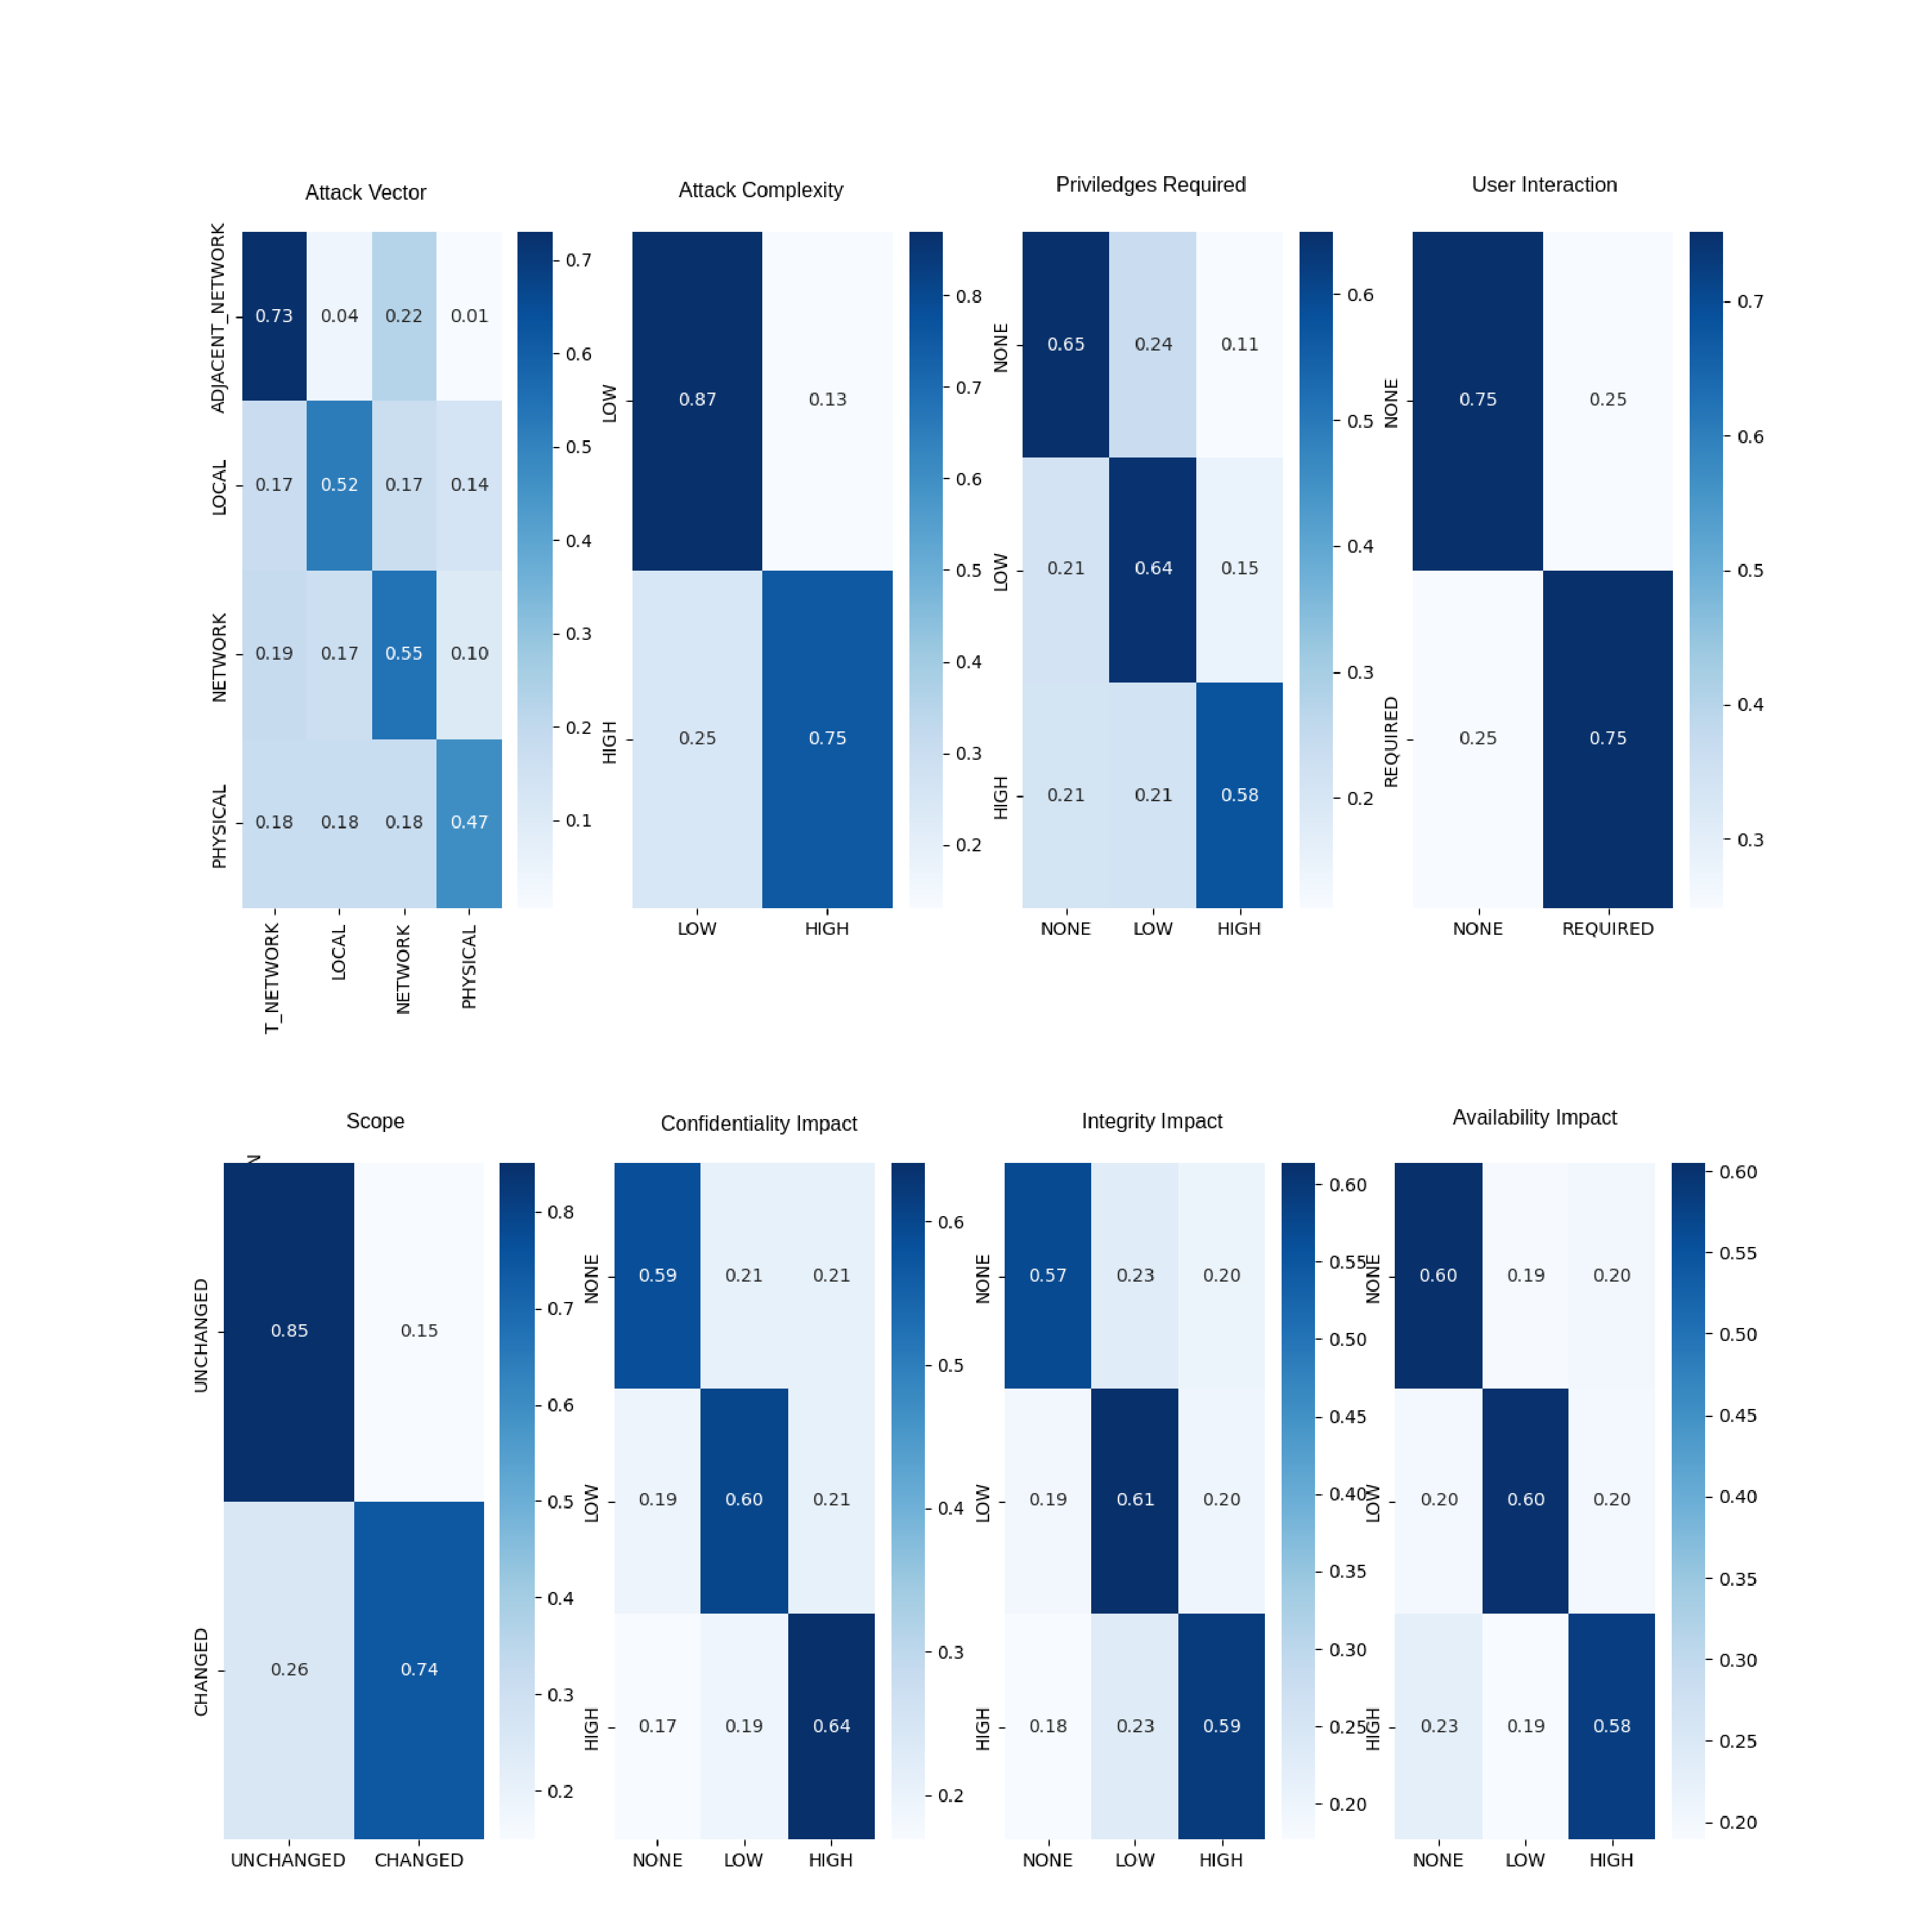
\includegraphics[width=1.5\textwidth]{figures/mitre_31_titles.pdf}}
	\caption{\label{fig:mitre_31_confusion_matrices}Confusion Matrices for MITRE for CVSS version 3.1}
\end{figure}

\begin{table}
	\label{fig:johnson_confusion_matrices}
	\centering
	\caption{Confusion Matrices for NVD on CVSS version 2.0 from Johnson et al.\@ \cite{bayes}}
	\[
		\begin{array}{c|c}
			\textbf{Access vector}  & \textbf{Access complexity} \\
			\hline
			\begin{tabular}{l|ccc}
				  & N    & A    & L    \\
				\hline
				N & 0.99 & 0    & 0    \\
				A & 0.21 & 0.71 & 0.08 \\
				L & 0.05 & 0.0  & 0.95 \\
			\end{tabular}
			                        &
			\begin{tabular}{l|ccc}
				  & L    & M    & H    \\
				\hline
				L & 0.54 & 0.29 & 0.17 \\
				M & 0.02 & 0.88 & 0.1  \\
				H & 0.01 & 0.08 & 0.91 \\
			\end{tabular}
			\\
			\textbf{Authentication} & \textbf{Confidentiality}   \\
			\hline
			\begin{tabular}{l|ccc}
				  & N    & S    & M    \\
				\hline
				N & 0.99 & 0.01 & 0    \\
				S & 0.04 & 0.95 & 0.01 \\
				M & 0.19 & 0.2  & 0.6  \\
			\end{tabular}
			                        &
			\begin{tabular}{l|ccc}
				  & C   & P    & N    \\
				\hline
				C & 0.4 & 0.2  & 0.2  \\
				P & 0.2 & 0.4  & 0.19 \\
				N & 0.2 & 0.21 & 0.4  \\
			\end{tabular}
			\\
			\textbf{Integrity}      & \textbf{Availability}      \\
			\hline
			\begin{tabular}{l|ccc}
				  & C    & P    & N    \\
				\hline
				C & 0.91 & 0.08 & 0.01 \\
				P & 0.05 & 0.93 & 0.02 \\
				N & 0.02 & 0.07 & 0.92 \\
			\end{tabular}
			                        &
			\begin{tabular}{l|ccc}
				  & C    & P    & N    \\
				\hline
				C & 0.92 & 0.07 & 0.01 \\
				P & 0.07 & 0.91 & 0.02 \\
				N & 0.02 & 0.11 & 0.87 \\
			\end{tabular}
		\end{array}
	\]
\end{table}

\subsection{CVSS Prediction}

Below, Table~\ref{tab:distil_part1} \& Table~\ref{tab:distil_part2} show the results of the
DistilBERT model trained on a combination of NVD and MITRE data. Unfortunately this has
a purely negative effect on all metrics, with the caveat that some of the standard deviations are
lower. Additional note is that the balanced accuracy for some metrics looks a bit weird, I believe that
is due to the model not outputing some of the categorical options for that metric. This applies to
all the balanced accuracy scores, apart from the Priorities Required (PR) and Confidentiality (C) as
seen on Table~\ref{tab:distil_part1} \& Table~\ref{tab:distil_part2}. As this
was done only recently I have not looked into this issue in-depth to see why this is happening, but
I will in the future. As to why the model performs worse, my theory is that the added data, and
therefore the overlapping CVEs with different scores confuse the model. I thought that adding the
additional data may have given the model a better chance of generalising, however this
does not appear to be the case.
The uncertainty between the two databases can serve as an indicator when
analyzing generated CVE scores. It suggests that the model may encounter similar challenges to those
faced by human evaluators. The lowest score for my model is in the Availability Impact
category, which is also low for Cody's model. This observation indicates a correlation between the
machine learning models' difficulties and the issues faced by human scorers. Attack Complexity also
presents challenges, likely due to data imbalance, as the dataset is heavily skewed towards the
\texttt{Low} score, thereby incentivizing the model to output \texttt{Low} scores (see
Figures~~\ref{fig:counts},~\ref{fig:nvd_31_confusion_matrices},~\ref{fig:mitre_31_confusion_matrices} for
reference).

\begin{table}[H]
	\centering
	\resizebox{\textwidth}{!}{%
		\begin{tabular}{llcccc}
			\toprule
			\textbf{Metric} & \textbf{Model}  & \textbf{AV}           & \textbf{AC}           & \textbf{PR}           & \textbf{UI}           \\
			\midrule
			\multirow{2}{*}{Accuracy}
			                & DistilBERT-Cody & \textbf{91.28 ± 0.26} & \textbf{95.64 ± 0.68} & \textbf{82.77 ± 0.24} & \textbf{93.86 ± 0.19} \\
			                & DistilBERT-Jake & 72.81 ± 0.32          & 92.62 ± 0.15          & 81.18 ± 0.18          & 66.35 ± 0.24          \\
			\midrule
			\multirow{2}{*}{F1}
			                & DistilBERT-Cody & \textbf{90.98 ± 0.31} & \textbf{93.85 ± 1.39} & \textbf{82.53 ± 0.26} & \textbf{93.82 ± 0.19} \\
			                & DistilBERT-Jake & 61.36 ± 0.42          & 89.08 ± 0.22          & 80.96 ± 0.19          & 52.93 ± 0.31          \\
			\midrule
			\multirow{2}{*}{Bal Acc}
			                & DistilBERT-Cody & \textbf{67.88 ± 2.11} & \textbf{55.82 ± 7.23} & \textbf{75.98 ± 0.47} & \textbf{92.46 ± 0.21} \\
			                & DistilBERT-Jake & 25.00 ± 0.00          & 50.00 ± 0.00          & 75.18 ± 0.31          & 50.00 ± 0.00          \\
			\bottomrule
		\end{tabular}
	}
	\caption{Comparison of the effects of the X pre-trained models on the CVSS v3.1 dataset (Part 1).}
	\label{tab:distil_part1}
\end{table}

\begin{table}[H]
	\centering
	\resizebox{\textwidth}{!}{%
		\begin{tabular}{llcccc}
			\toprule
			\textbf{Metric} & \textbf{Model}  & \textbf{S}            & \textbf{C}            & \textbf{I}            & \textbf{A}            \\
			\midrule
			\multirow{2}{*}{Accuracy}
			                & DistilBERT-Cody & \textbf{96.38 ± 0.09} & \textbf{86.24 ± 0.20} & \textbf{87.15 ± 0.10} & \textbf{88.70 ± 0.10} \\
			                & DistilBERT-Jake & 80.21 ± 0.16          & 82.45 ± 0.11          & 45.71 ± 0.26          & 52.53 ± 0.23          \\
			\midrule
			\multirow{2}{*}{F1}
			                & DistilBERT-Cody & \textbf{96.30 ± 0.10} & \textbf{86.09 ± 0.21} & \textbf{87.11 ± 0.10} & \textbf{88.04 ± 0.11} \\
			                & DistilBERT-Jake & 71.40 ± 0.22          & 82.34 ± 0.12          & 28.68 ± 0.28          & 36.18 ± 0.27          \\
			\midrule
			\multirow{2}{*}{Bal Acc}
			                & DistilBERT-Cody & \textbf{91.57 ± 0.43} & \textbf{82.70 ± 0.36} & \textbf{85.81 ± 0.10} & \textbf{64.01 ± 0.13} \\
			                & DistilBERT-Jake & 50.00 ± 0.00          & 79.85 ± 0.23          & 33.33 ± 0.00          & 33.33 ± 0.00          \\
			\bottomrule
		\end{tabular}
	}
	\caption{Comparison of the effects of the X pre-trained models on the CVSS v3.1 dataset (Part 2).}
	\label{tab:distil_part2}
\end{table}


\section{Discussion}\label{discussion}

% \subsubsection*{Case Study: Curl Library Vulnerability}

% A practical example of the issues with CVSS scoring can be seen with a vulnerability in the curl
% library~\cite{curl_library}. The vulnerability was described as an integer overflow in
% \texttt{tool\_operate.c}, which could result in undefined behaviour if a user entered a value
% exceeding the integer limit~\cite{curlcve}. Initially, this vulnerability received a CVSS score of
% 9.8. Daniel Stenberg, the original founder of curl, disagreed with this high score, arguing that it
% was a bug fixed back in 2019~\cite{curl1}. Despite his efforts, the CVE (Common Vulnerabilities and
% Exposures) entry remained. Stenberg successfully disputed the score and NVD lowered the score to
% 3.3~\cite{curl2}. Stenberg was eventually somewhat successful in mitigating this issue, however it
% took a good chunk of his valuable time, as well as all others involved. This example highlights the
% time-consuming nature of rectifying CVSS scores and the potential for initial misratings.


\subsubsection{Exploit Prediction Scoring System}

EPSS is developed by FIRST, the same group who govern the CVSS standard. It has a different take
on the problem, focusing on a data driven model designed to give \say{a daily estimate of the probability
	of exploitation activity being observed over the next 30 days~\cite{EPSS}.} If the data shown on the model
page is to be believed, it is a promising system (some of their findings Figure~\ref{fig:epss_and_cvss},
Figure~\ref{fig:epss}). Unfortunately, while good to keep in mind for the industry, it is less useful
for our purposes. This is a pretrained and uninterpretable model, from the outside at least.
Analysis could be done on the output of the model in relation to CVEs, but that will not be a focus
going forward.


\subsection{Future Work}

Despite the disadvantages of CVSS, I will continue to focus on it in my studies. My focus will pivot
towards the interpretability of large language models, particularly from the perspective of data.
The CVE dataset is messy, with many poorly written CVE descriptions that are not useful for machine
learning models. I plan to clean up this dataset by identifying and removing low-quality entries. To
achieve this, I will perform clustering and general analysis of the CVE descriptions to better
understand the dataset and develop heuristics for filtering it.

\section{Conclusion}

The Common Vulnerability Scoring System (CVSS) is integral in prioritizing and managing the
ever-growing number of software vulnerabilities. While the current approach heavily relies on
manually assigned scores from the National Vulnerability Database (NVD), it may be worth using the
MITRE database as well. However, the findings are very much inconclusive, it is possible that adding
the extra data during model training is worth it, but so far it has only been to the detriment of
performance. One key issue is the variability in CVSS scores between different databases, such as NVD
and MITRE, which suggests a lack of consistency in the scoring process. This inconsistency can
confuse automated systems and reduce the overall reliability of the predicted scores.

In conclusion, while CVSS remains a crucial tool for vulnerability management, its current
implementation has limitations that need to be addressed. The integration of machine learning models
offers a promising solution to automate and enhance the accuracy of CVSS scoring. However the focus
should be on predicting the distinct categorical variable for each metric, as this is a universally
interesting classification task and will be more able to apply to changes in the CVSS standard.
Future research should focus on refining these models, and focusing on interpretability, whether
through LLM interpretability methods, or through more traditional databased clustering.

\printbibliography[title={References}]



\appendix

\renewcommand{\thesection}{Appendix \Alph{section}}

\subsection{CVSS figures from other versions}

Below is a collection of confusion matrics which are results from the Bayesian analysis of CVSS
versions 2.0 \& 3.0 for both the NVD and MITRE databases. Version 2.0 for MITRE is especially rough
as there was very little data.

\begin{figure}[H]
	\centering
	\makebox[\textwidth][c]{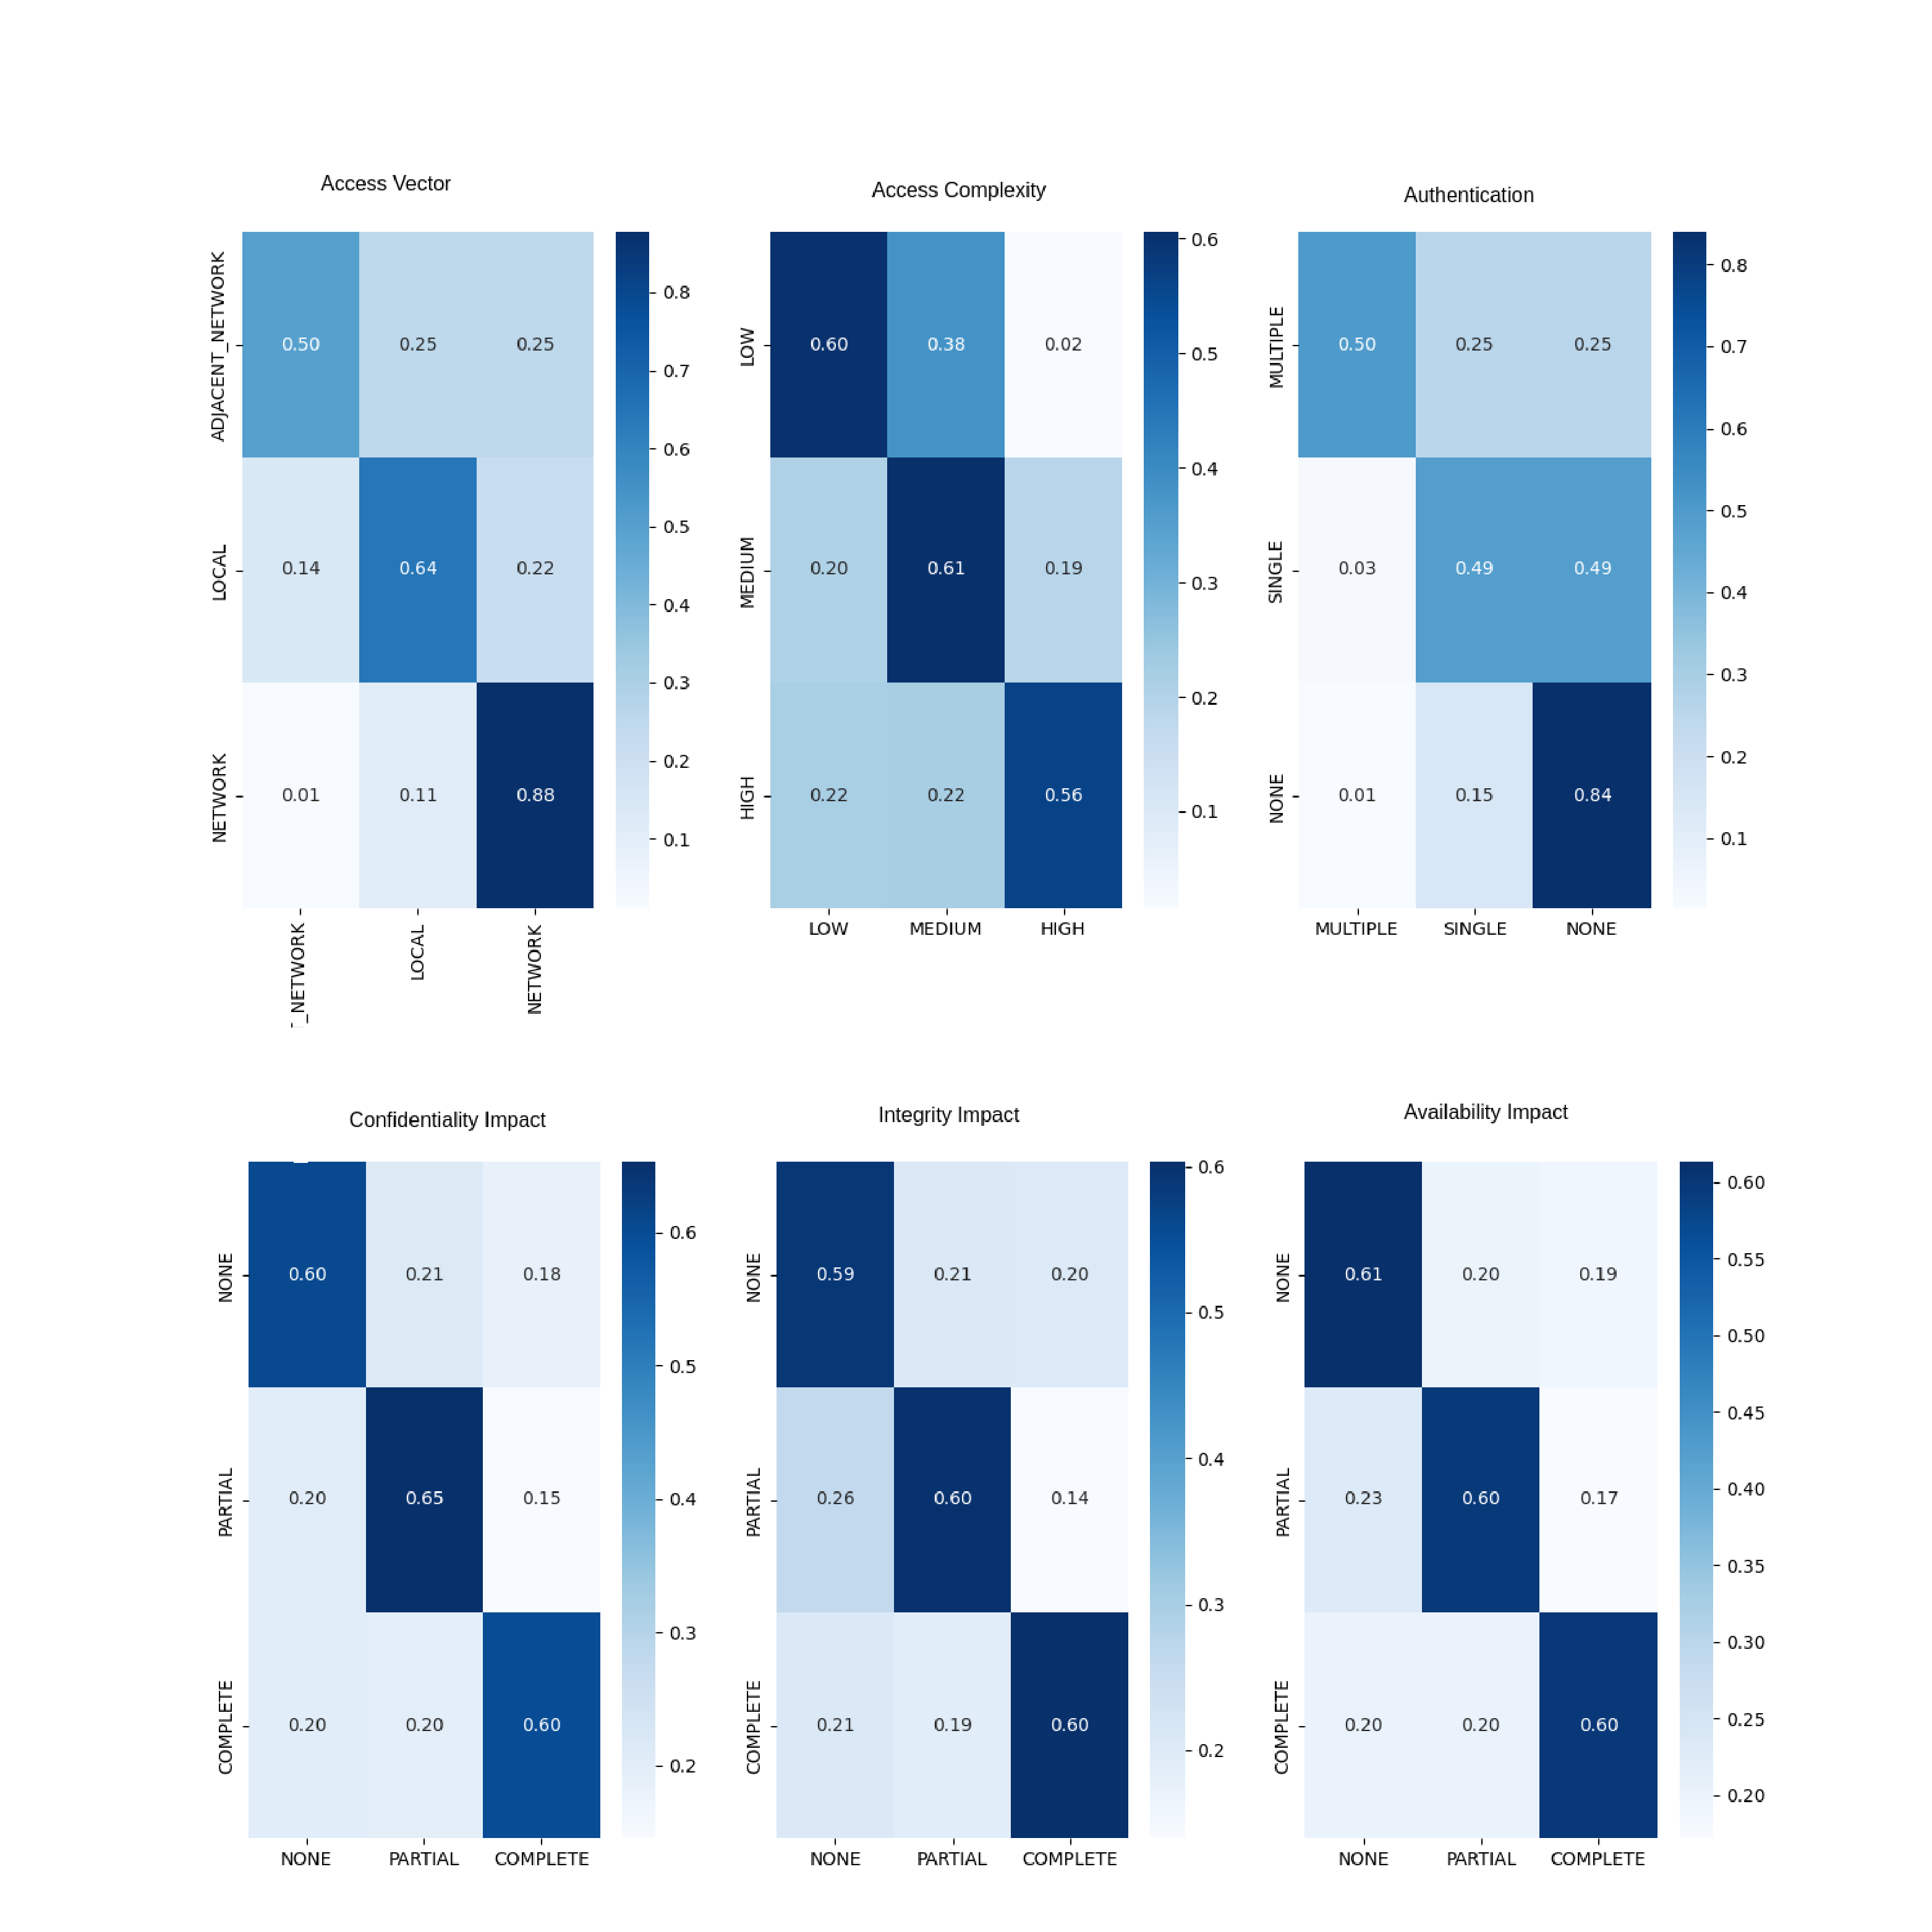
\includegraphics[width=1.5\textwidth]{{figures/nvd_2_titles.pdf}}}%
	\caption{\label{fig:nvd_2_confusion_matrices}Confusion matrix of estimated accuracy for CVSS metrics for version 2.0 for NVD}
\end{figure}

\begin{figure}[H]
	\centering
	\makebox[\textwidth][c]{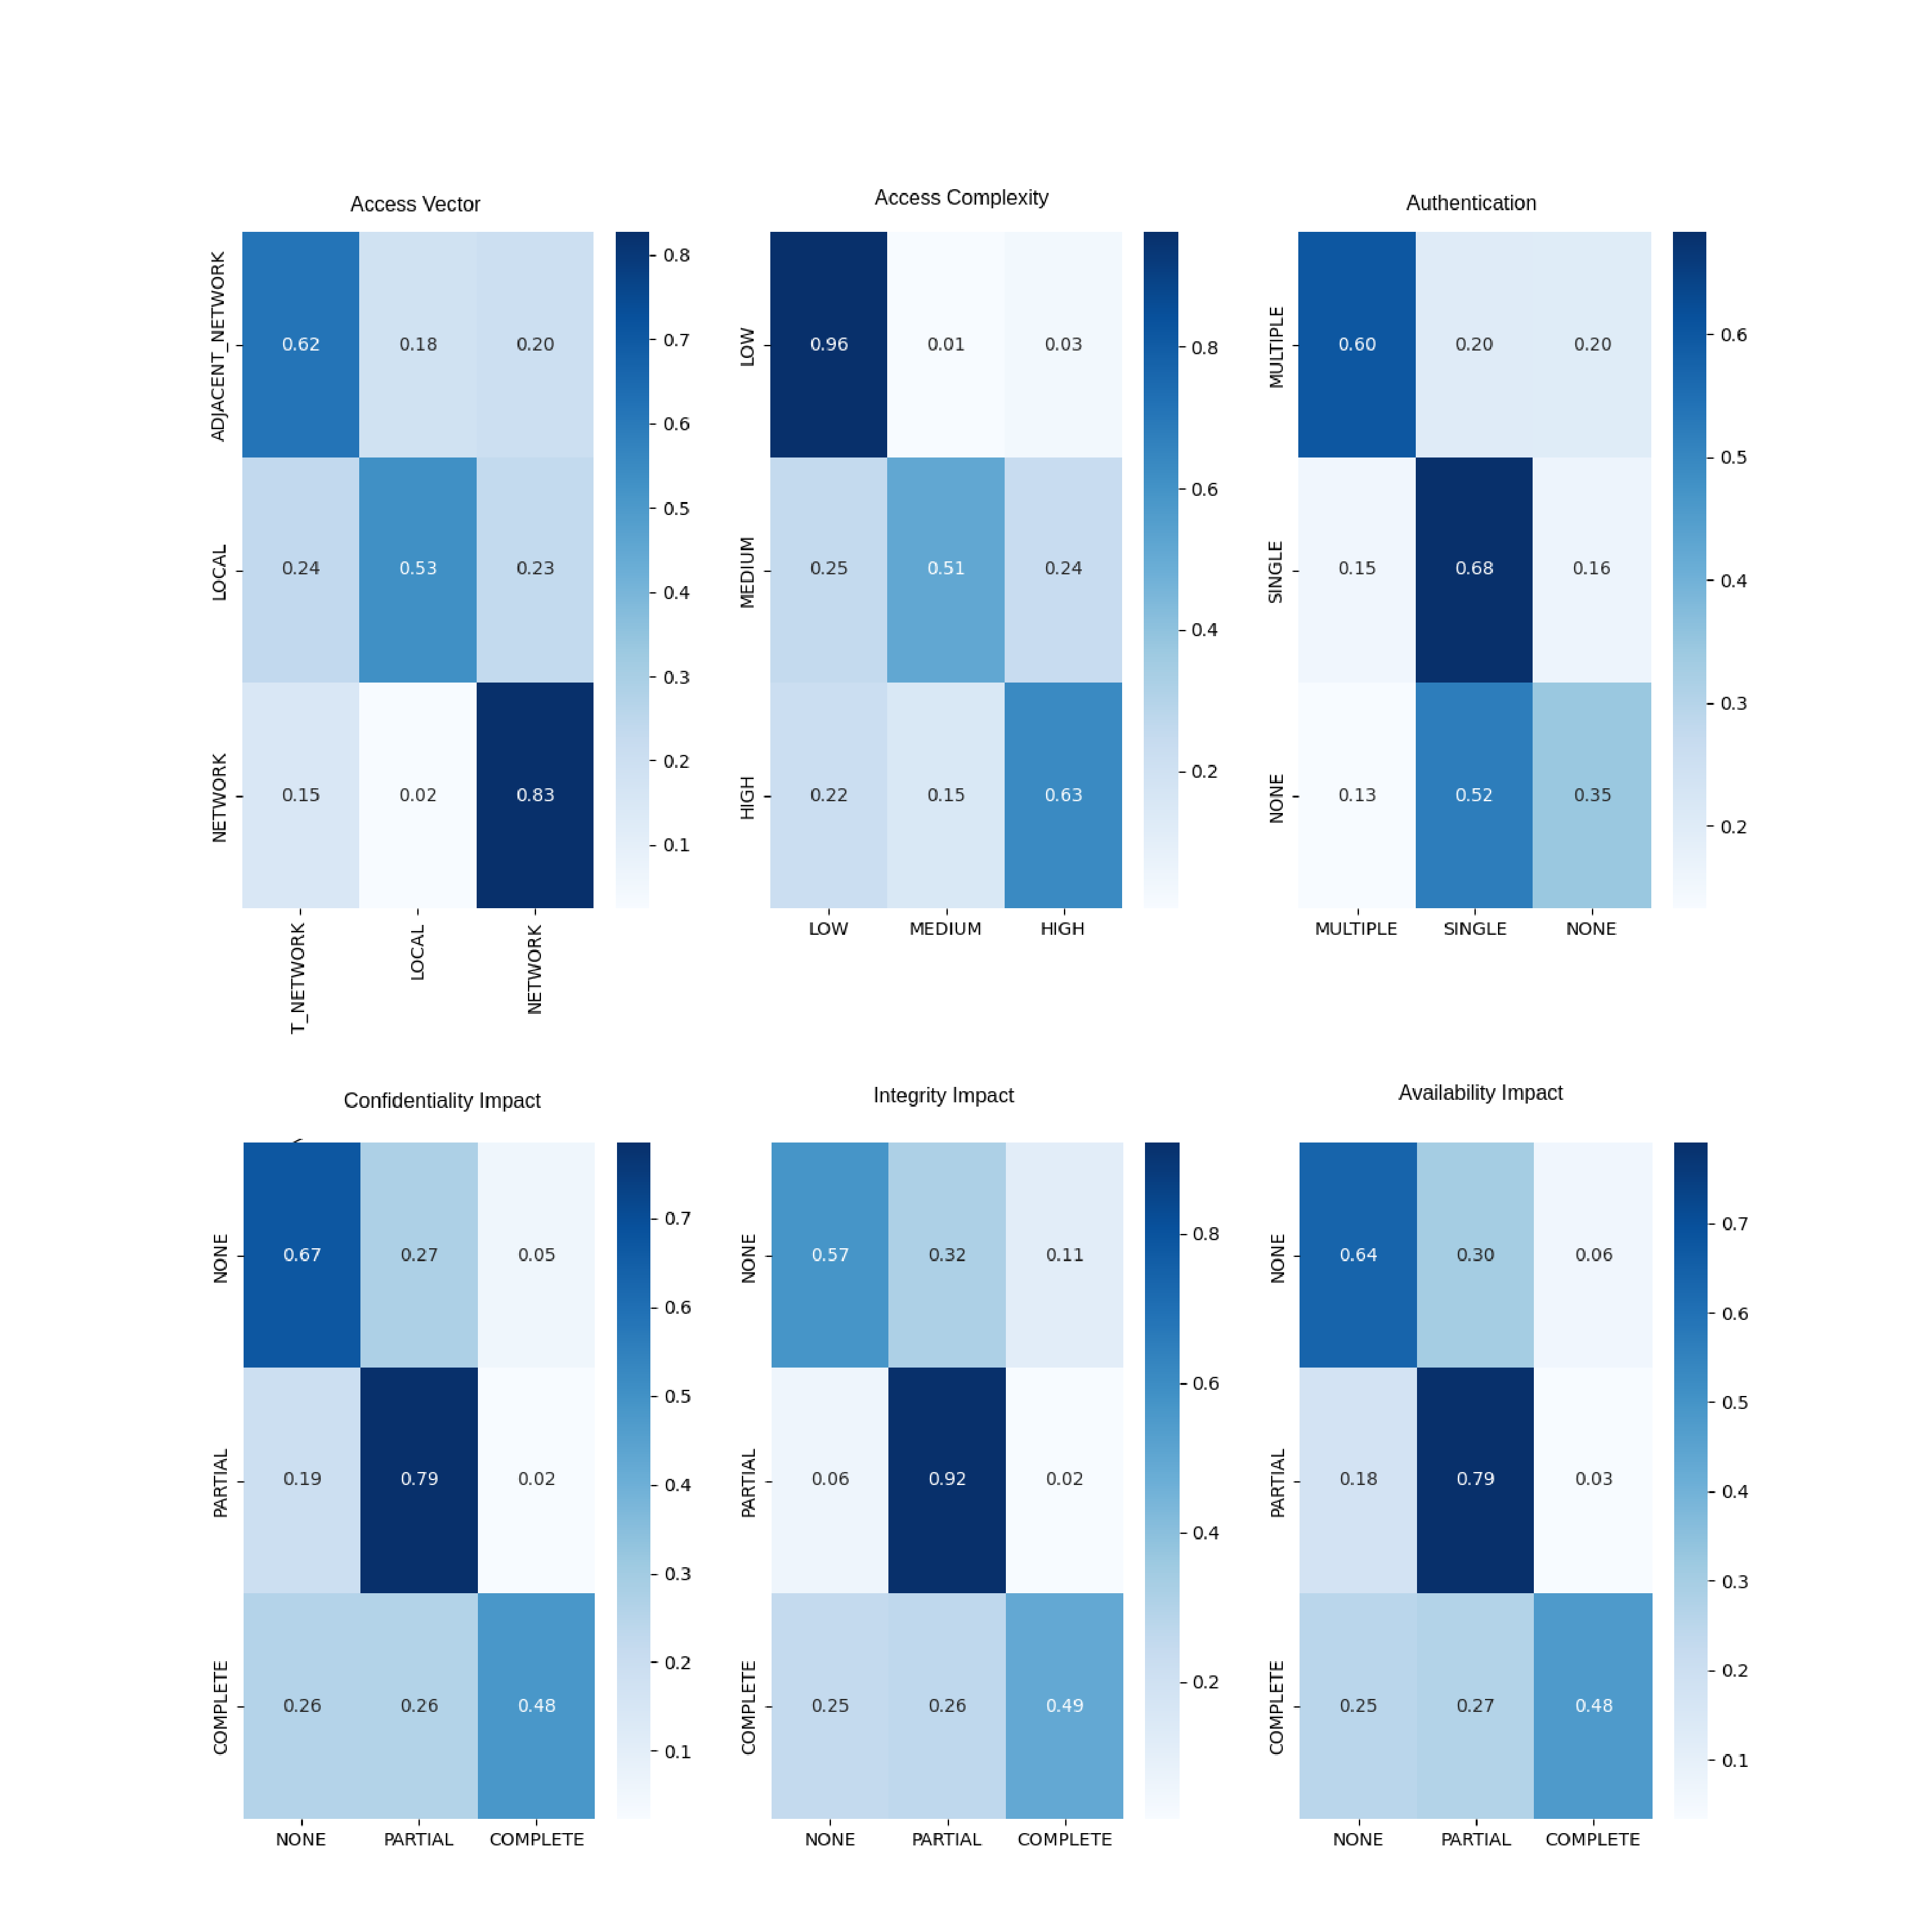
\includegraphics[width=1.5\textwidth]{figures/mitre_2_titles.pdf}}
	\caption{\label{fig:mitre_2_confusion_matrices}Confusion matrix of estimated accuracy for CVSS
		metrics for version 2.0 for MITRE}
\end{figure}

\begin{figure}[H]
	\centering
	\makebox[\textwidth][c]{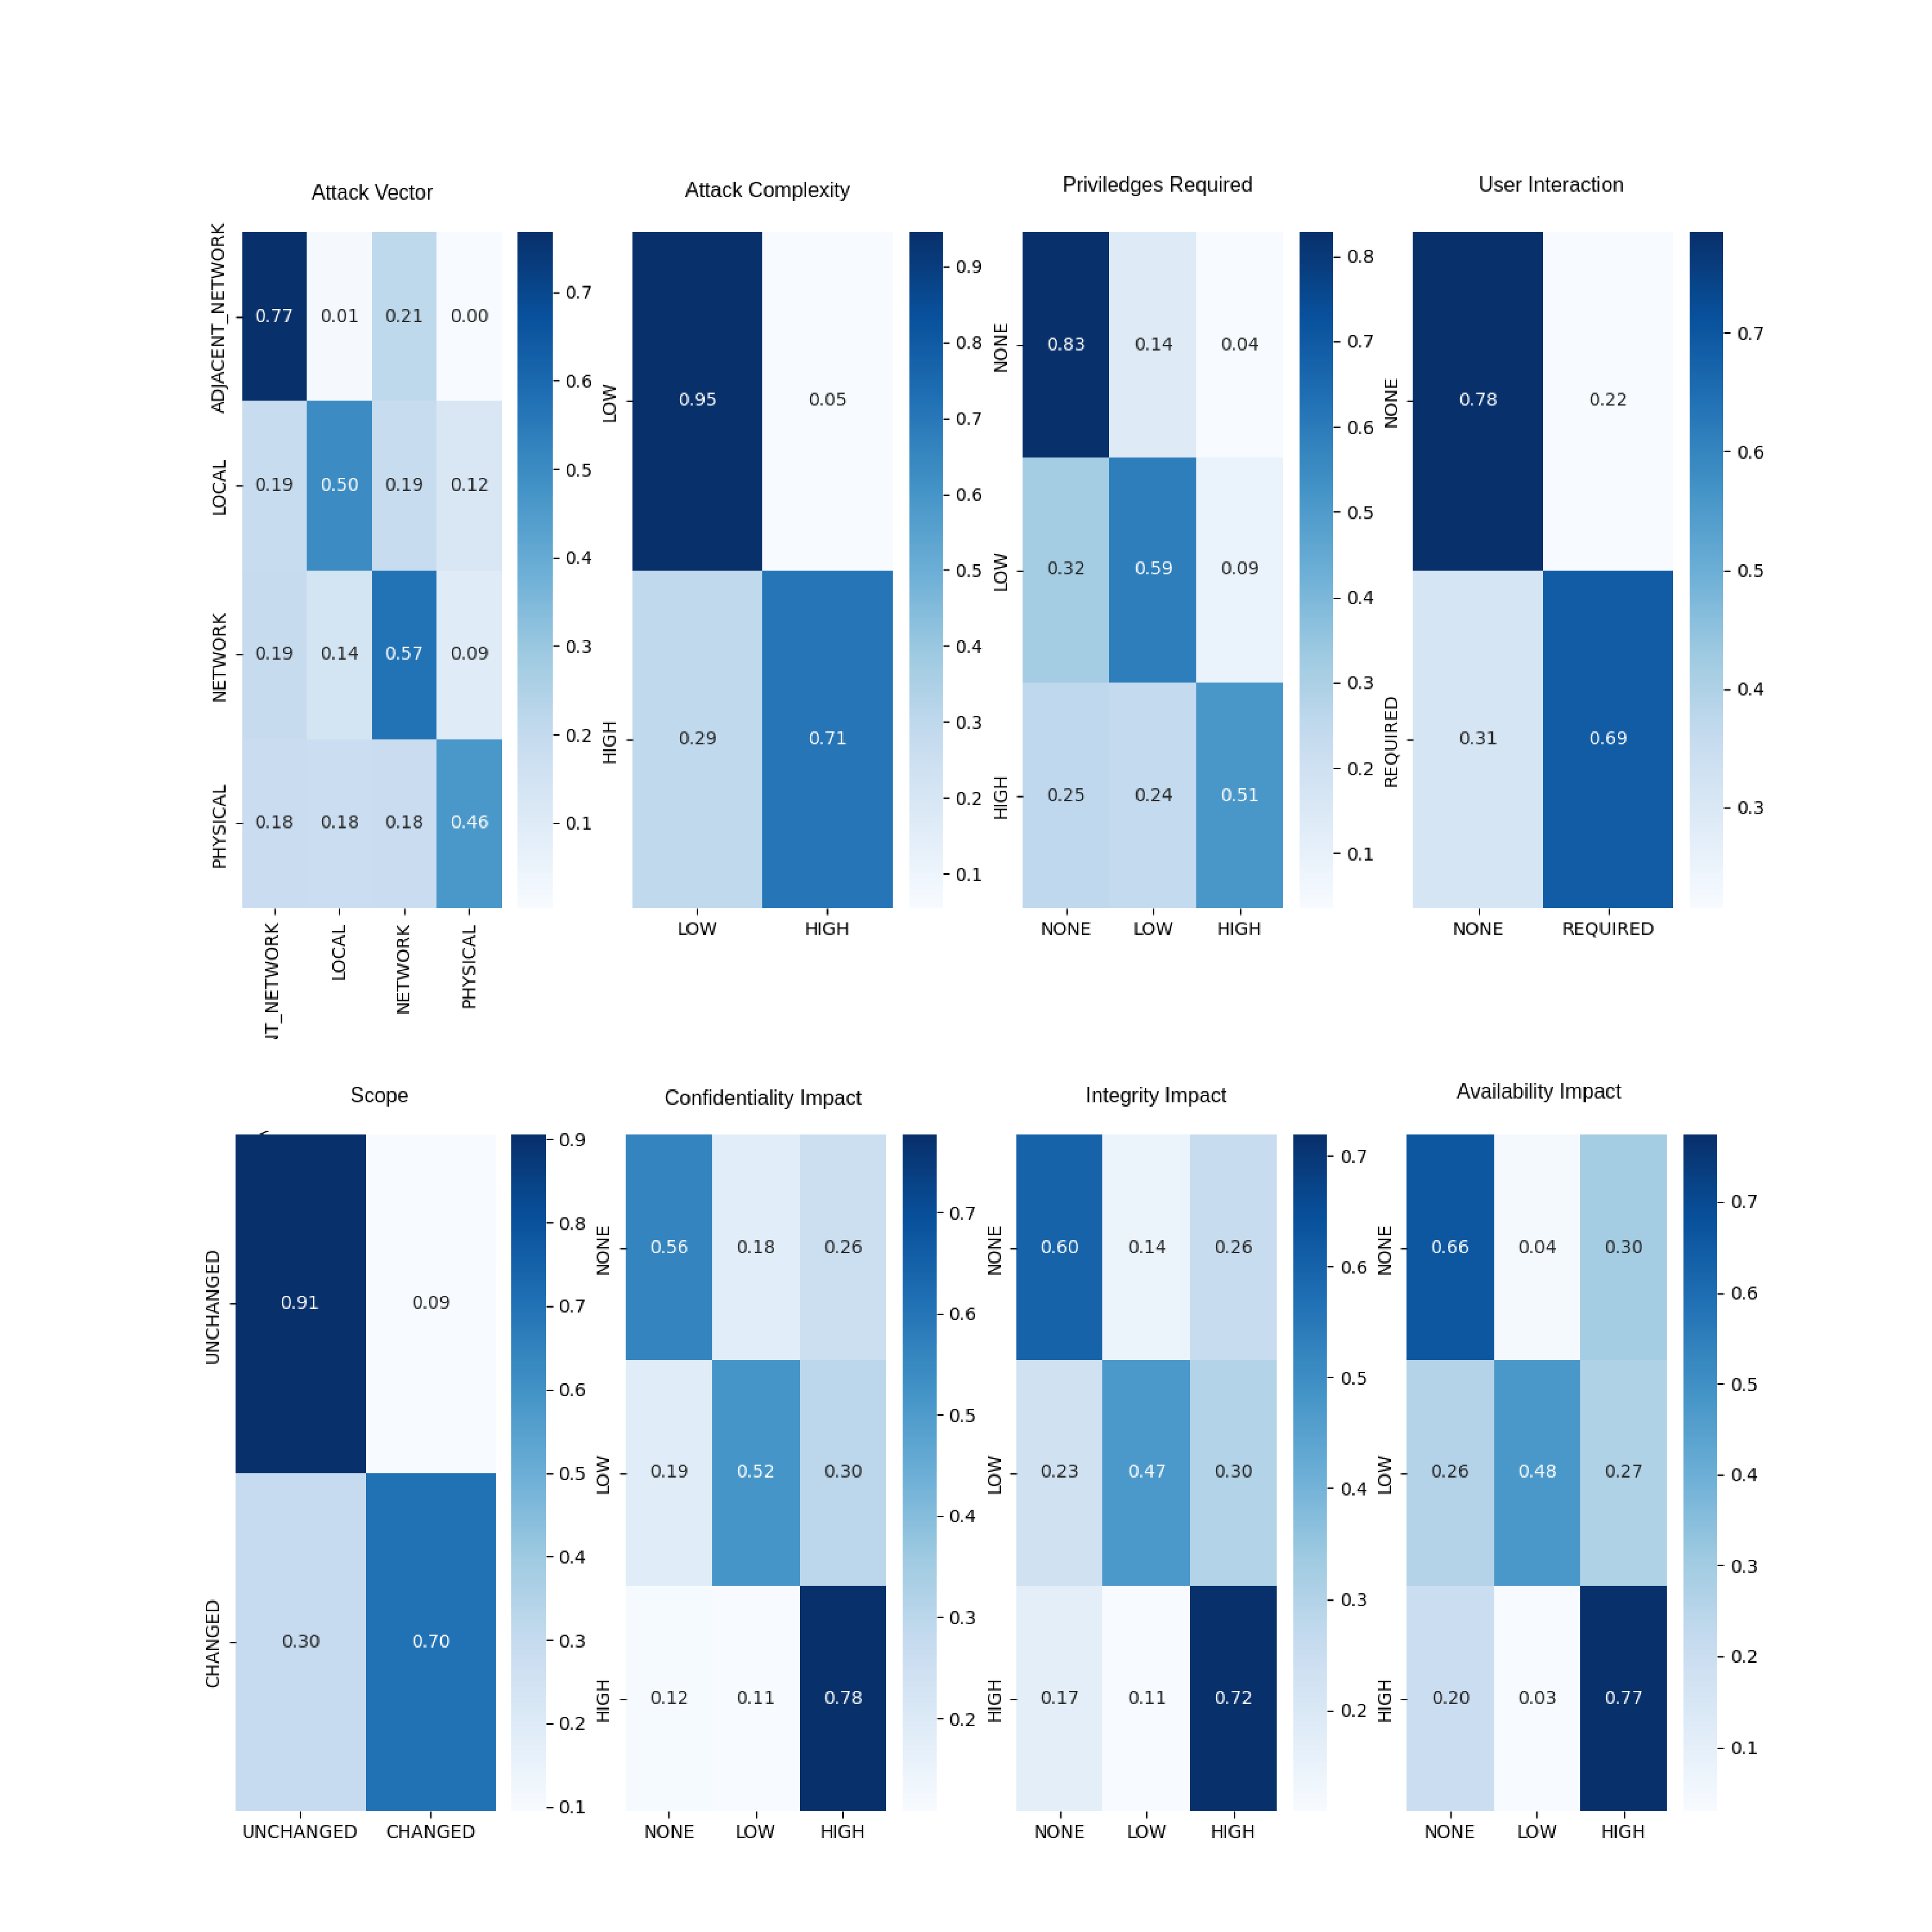
\includegraphics[width=1.5\textwidth]{figures/nvd_30_titles.pdf}}
	\caption{\label{fig:nvd_30_confusion_matrices}Confusion matrix of estimated accuracy for CVSS metrics for version 3.0 for NVD}
\end{figure}

\begin{figure}[H]
	\centering
	\makebox[\textwidth][c]{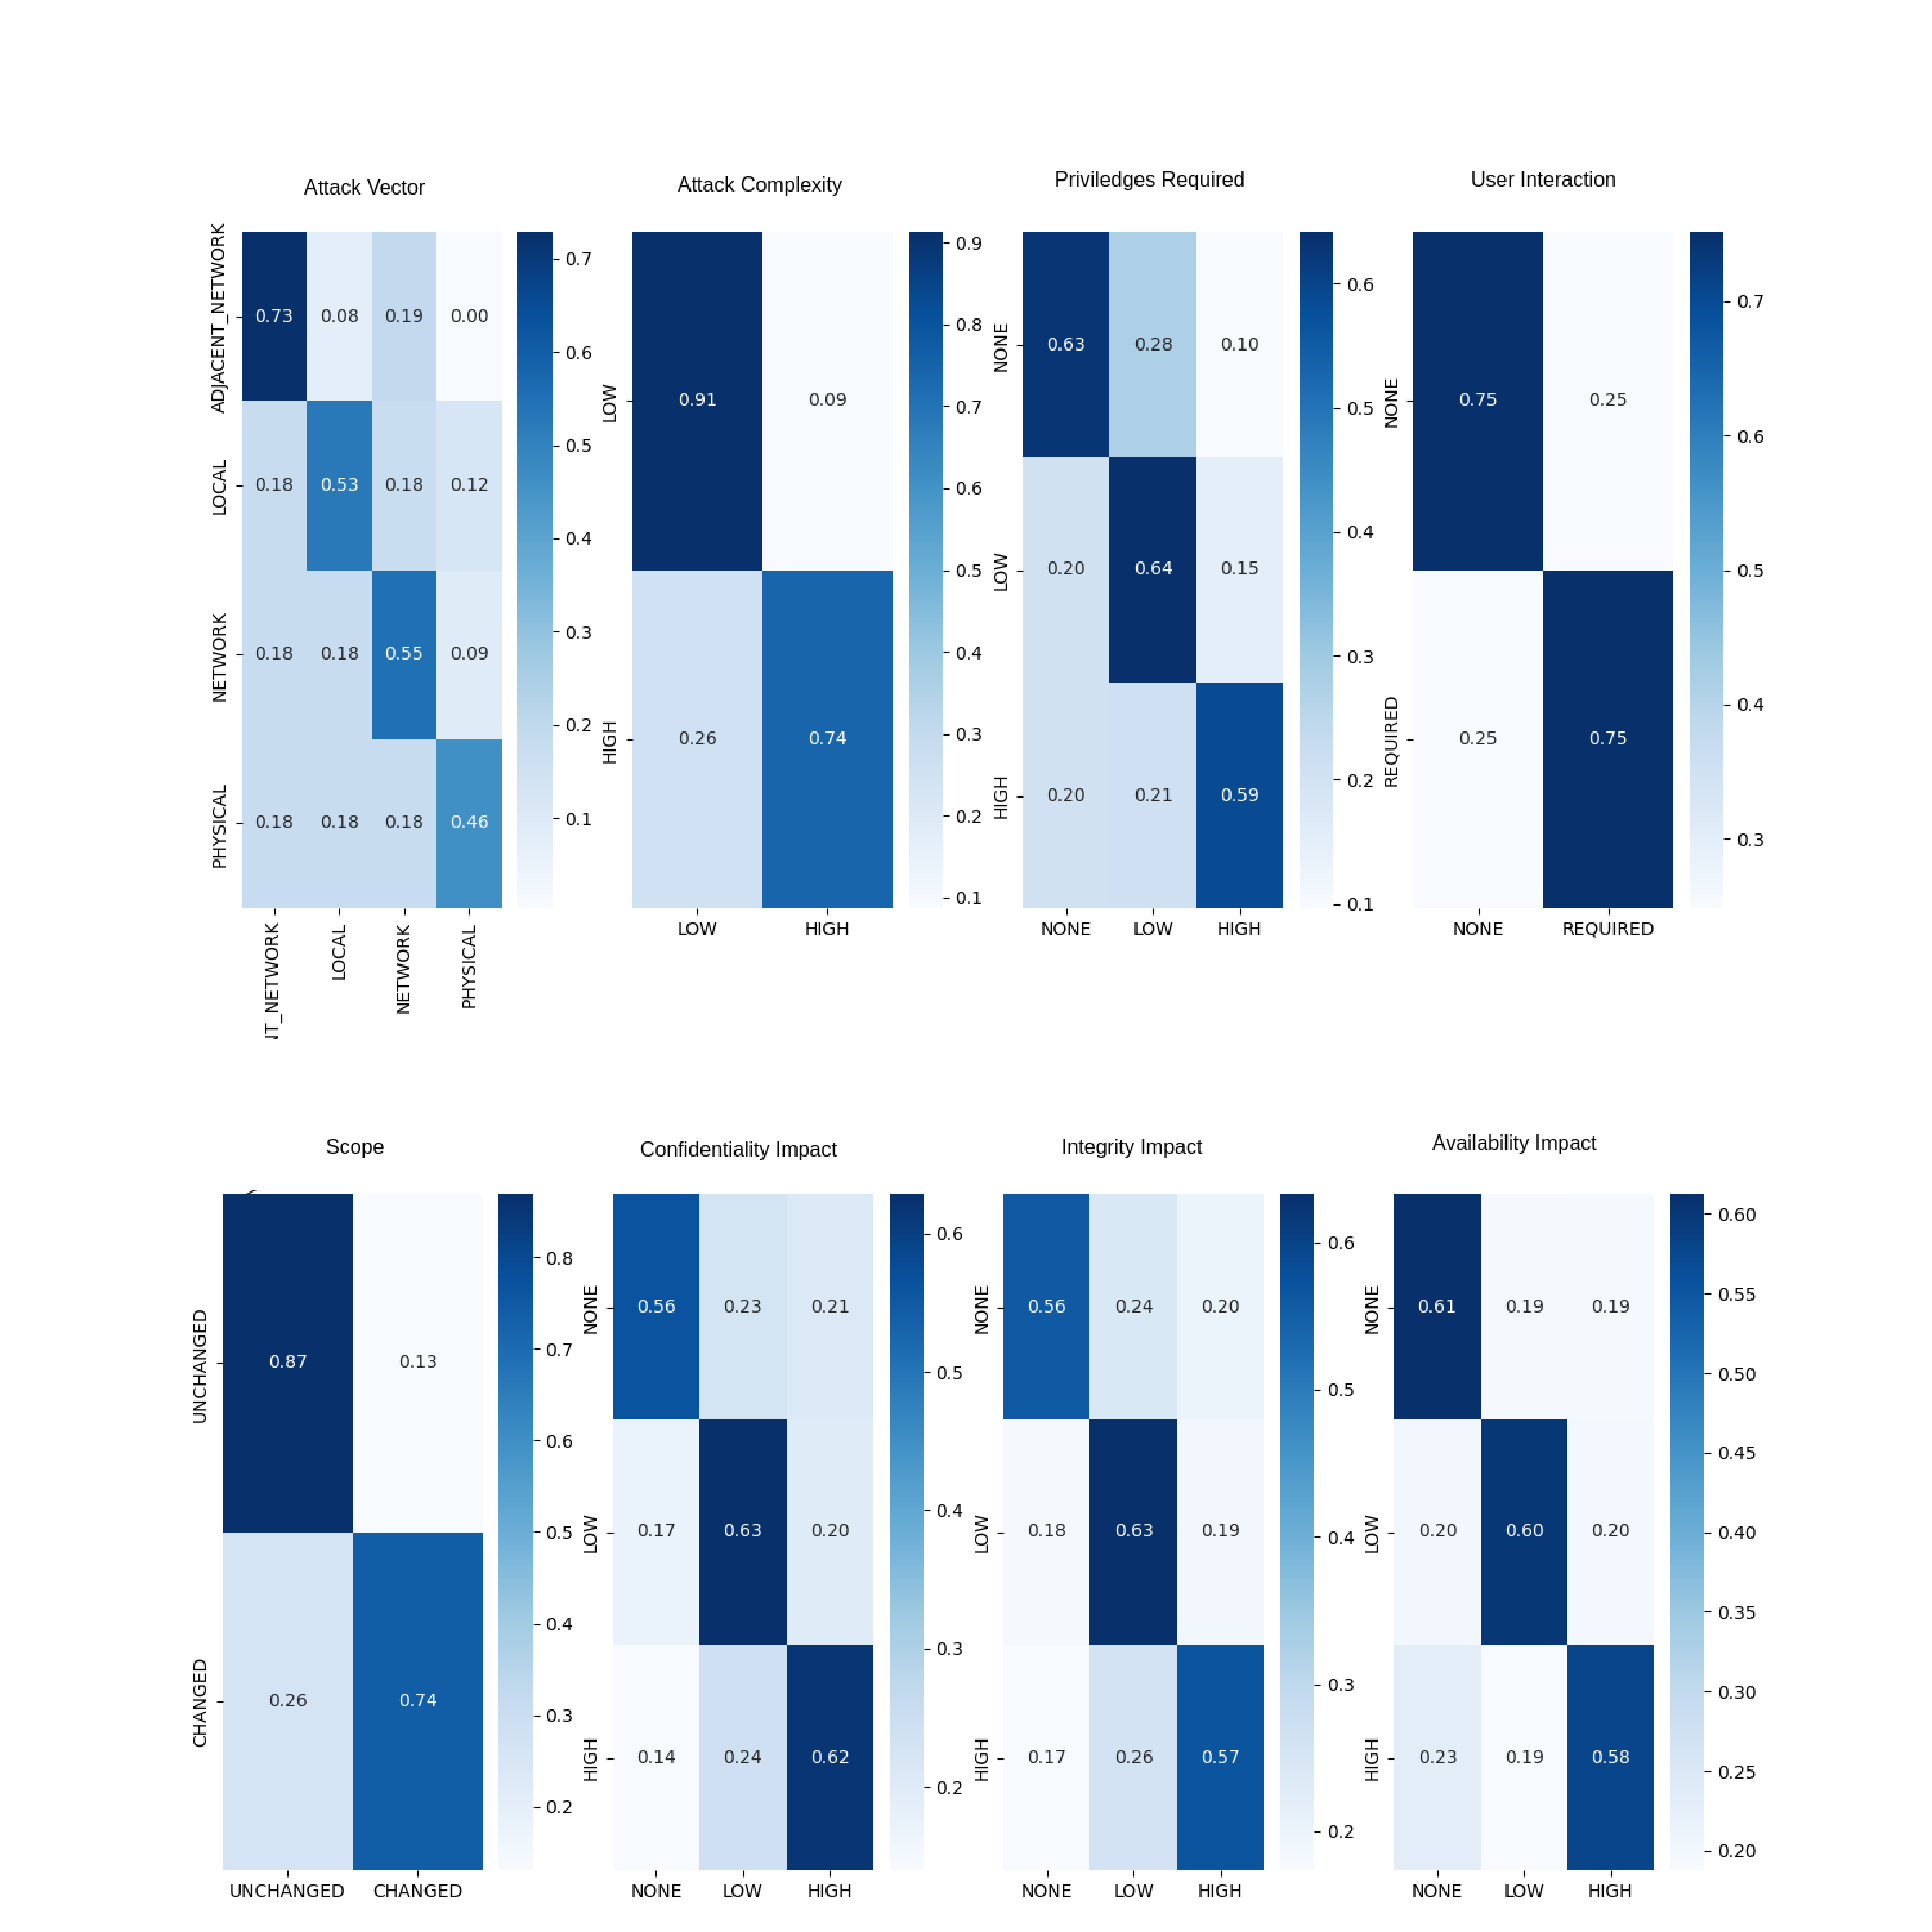
\includegraphics[width=1.5\textwidth]{figures/mitre_30_titles.pdf}}
	\caption{\label{fig:mitre_30_confusion_matrices}Confusion matrix of estimated accuracy for CVSS
		metrics for version 3.0 for MITRE}
\end{figure}



\subsection{CVSS 3.1 Base Score formula} \label{equation}

Below is a formulaic representation of the CVSS 3.1 base score formula.
	{\scriptsize
		\begin{equation}
			ISS = 1 - ((1 - Confidentiality) \times (1 - Integrity) \times (1 - Availability)) \\
		\end{equation}
		\begin{equation}
			Impact =
			\begin{cases}
				7.52 \times (ISS - 0.029) - 3.25 \times (ISS - 0.02)^{15} & \text{if \textit{Scope} is
				\textit{Changed}}                                                                      \\
				6.42 \times ISS                                           & \text{if \textit{Scope} is
					\textit{Unchanged}}
			\end{cases}
		\end{equation}

		\begin{equation}
			Exploitability = 8.22 - AttackVector \times AttackComplexity \times PrivilegesRequired \times
			UserInteraction \\
		\end{equation}

		\begin{equation}
			Base Score =
			\begin{cases}
				0                                                           & Impact \leq 0              \\
				Roundup(Minimum(1.08 \times (Impact + Exploitability), 10)) & \text{if \textit{Scope} is
				\textit{Changed}}                                                                        \\
				Roundup(Minimum((Impact + Exploitability), 0))              & \text{if \textit{Scope} is
				\textit{Unchanged}}                                                                      \\
			\end{cases}
		\end{equation}
	}

\subsection{Exploit Prediction Scoring System diagrams for reference}

Below are two graphs from FIRST, the creator of EPSS. These show some of the results they have
found for this system, especially when comparing EPSS to CVSS in terms of effeciency of effort if
you use EPSS to guide remediation of vulnerabilities.

\begin{figure}
	\centering
	\makebox[\textwidth][c]{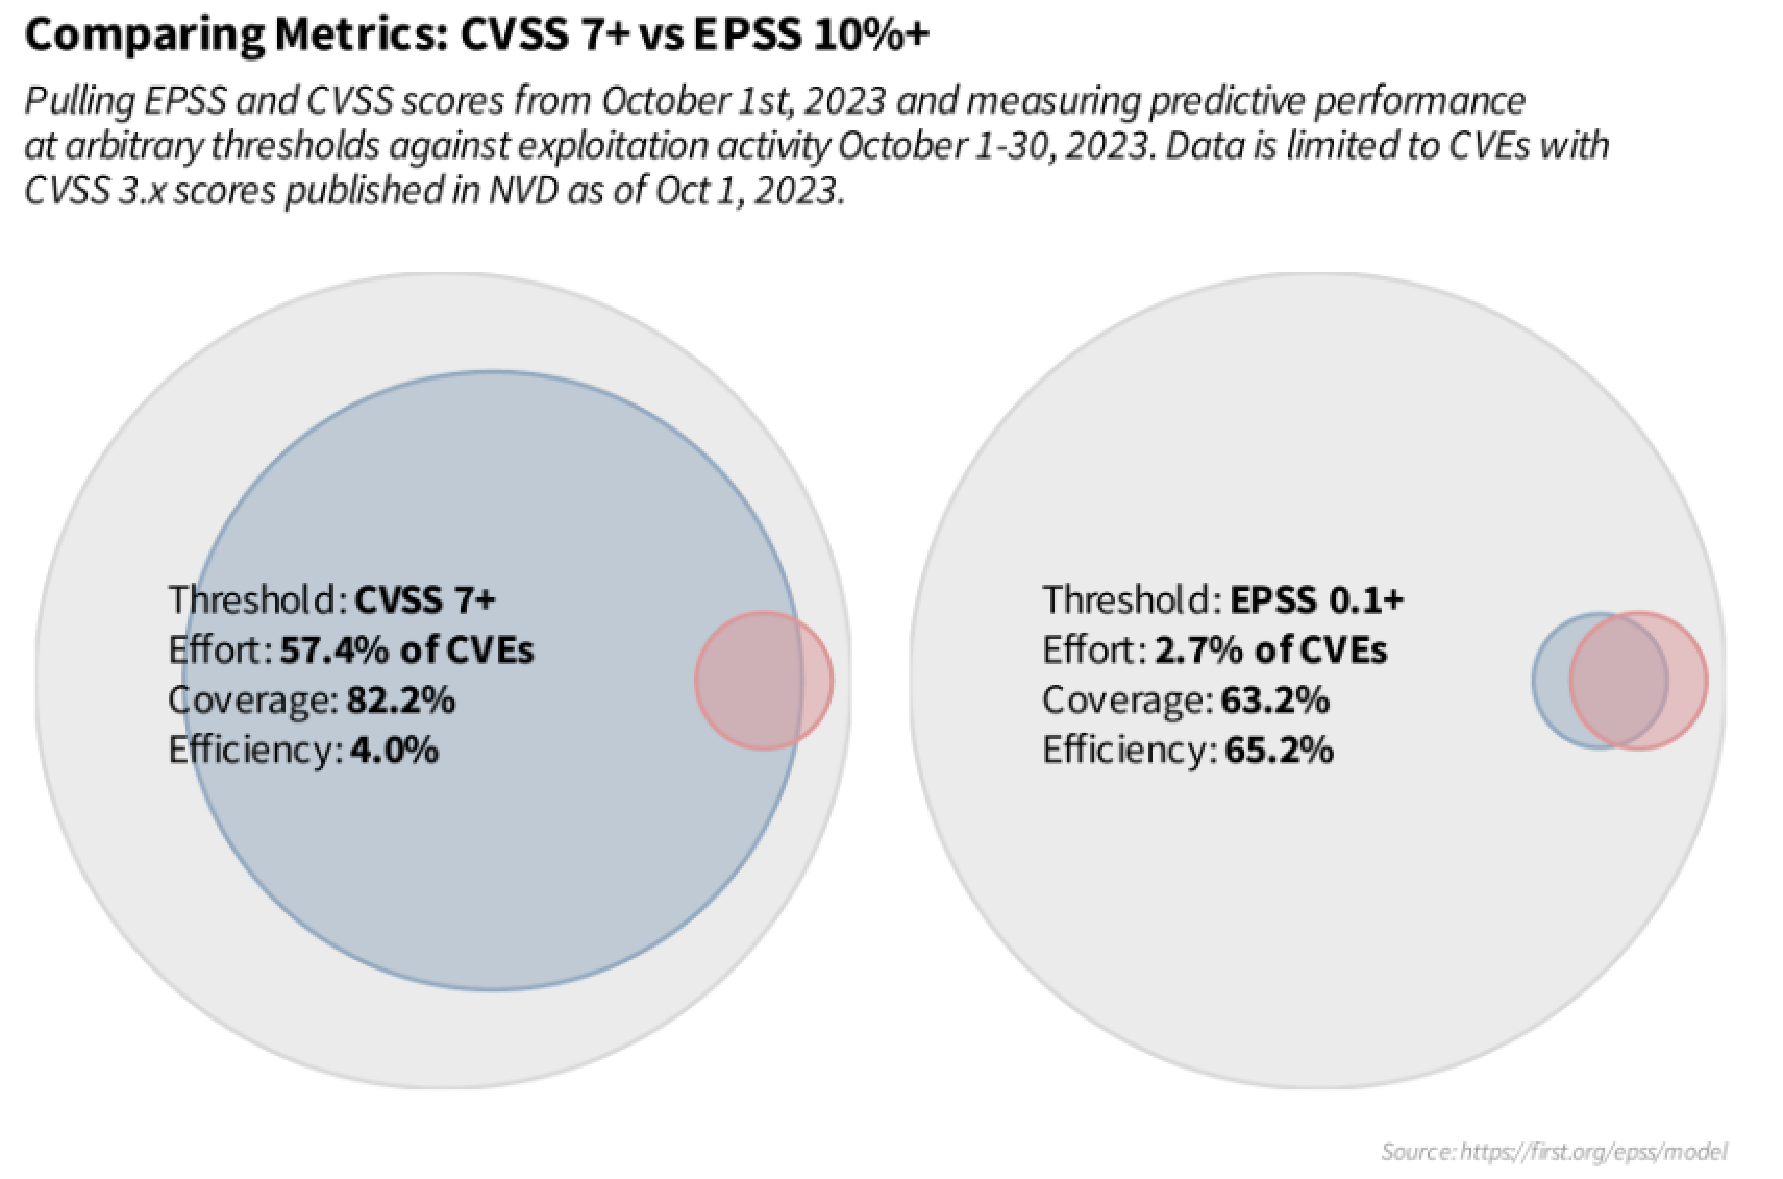
\includegraphics[width=1\textwidth]{figures/epss.pdf}}
	\caption{\label{fig:epss}Comparing Metrics: CVSS 7+ vs. EPSS 10\%+ sourced from \cite{EPSS}}
\end{figure}

\begin{figure}
	\centering
	\makebox[\textwidth][c]{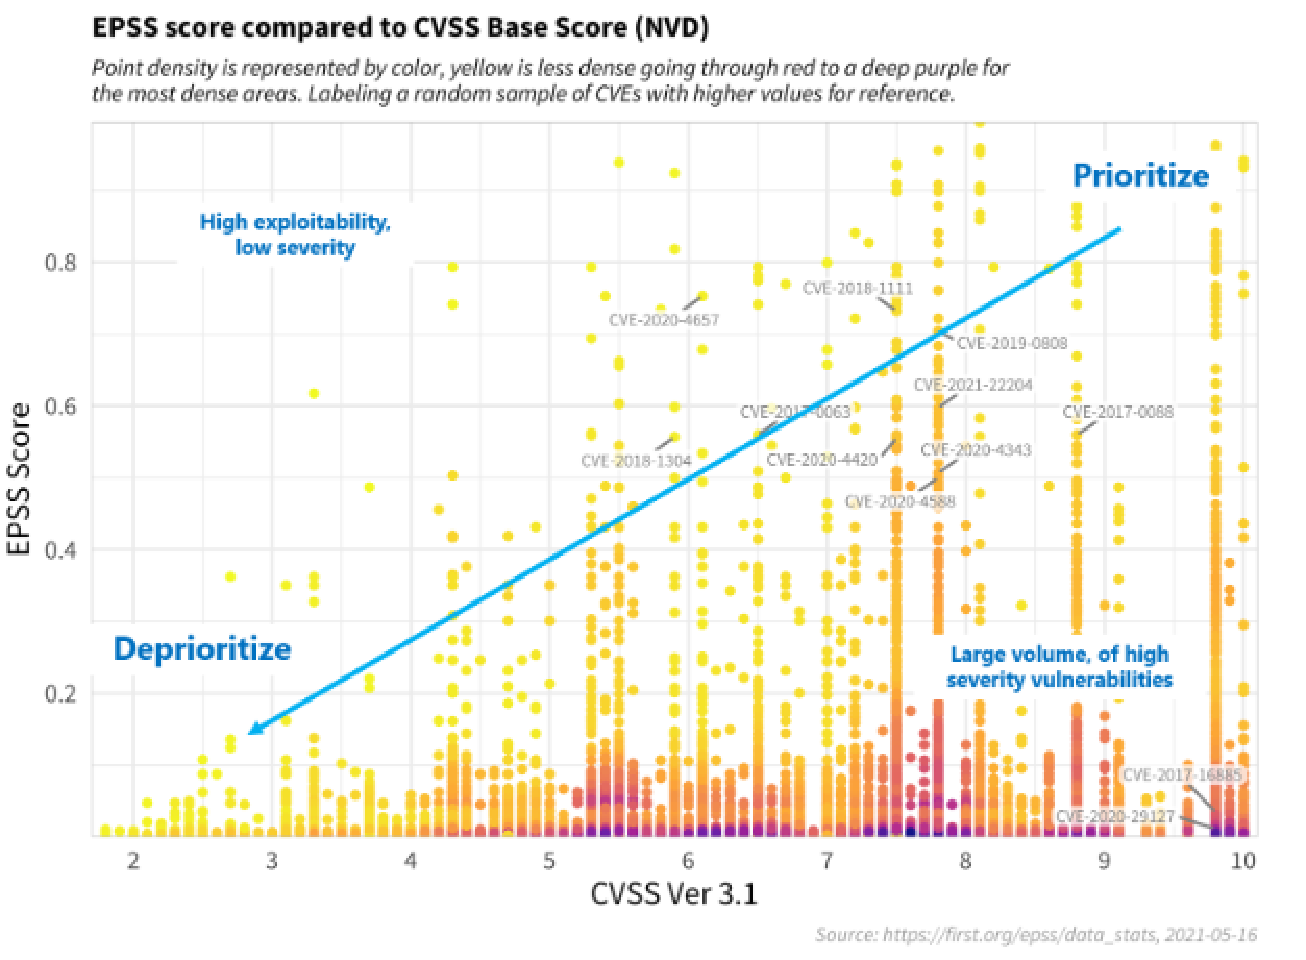
\includegraphics[width=1\textwidth]{figures/epss_and_cvss.pdf}}
	\caption{\label{fig:epss_and_cvss}EPSS score compared to CVSS Base Score (NVD) sourced from
		\cite{EPSS_USER}}
\end{figure}

\section{Aims and Objectives}

\subsection*{Original}

\paragraph{Aims}
The primary aim of this research is to develop sophisticated predictive models capable of accurately determining
the severity levels of security threats based on the CVSS. This will involve a comprehensive review and comparison
of current datasets, with a focus on leveraging natural language descriptions provided in security vulnerability reports.
The project intends to utilize advanced transformer-based models to achieve this goal, contributing to the field of
cybersecurity by enhancing the precision of threat severity assessments.

\paragraph{Objectives}
\begin{itemize}[noitemsep]
	\item Conduct a comprehensive literature review to understand the current landscape of CVSS score prediction and the methodologies employed in existing models.
	\item Replicate successful methodologies to verify the accuracy of CVSS score databases, with a particular focus on alignment with recent CVSS standards and datasets.
	\item Explore opportunities for enhancing existing methodologies, including the investigation of data amalgamation from multiple databases to ascertain improvements in model performance.
	\item Experiment with various model architectures to identify the most effective approach in terms of predictive accuracy, specifically focusing on metrics such as the F1 score and balanced accuracy.
\end{itemize}

\paragraph{Timeline}
\begin{itemize}[noitemsep]
	\item March: Initiate the project with a literature review, system environment setup, and resource gathering.
	\item March-April: Replicate existing methodologies to validate findings and ensure alignment with current standards.
	\item May-June: Generate preliminary results and compile an interim report detailing findings and methodologies.
	\item July-August: Conduct experiments with various data source combinations and model architectures to identify optimal configurations.
	\item September-October: Finalize experimental work, analyze results, and prepare the comprehensive final report.
\end{itemize}

\subsection*{Revised}

\paragraph{Aims}

The primary aim of this research is to develop sophisticated predictive models capable of accurately determining
the severity levels of security threats based on the CVSS. This will involve a comprehensive review and comparison
of current datasets, with a focus on leveraging natural language descriptions provided in security vulnerability reports.
The project intends to utilize advanced transformer-based models to achieve this goal, contributing to the field of
cybersecurity by enhancing the precision of threat severity assessments.

\paragraph{Objectives}
\begin{itemize}[noitemsep]

	\item Conduct a comprehensive literature review to understand the current landscape of CVSS
	      score prediction and the methodologies employed in existing models.

	\item Replicate successful methodologies to verify the accuracy of CVSS score databases, with a
	      particular focus on alignment with recent CVSS standards and datasets.

	\item Explore opportunities for enhancing existing methodologies, including the investigation of
	      data amalgamation from multiple databases to ascertain improvements in model performance.

	\item Look into data cleaning and clustering, to improve the efficacy of the models, as well as
	      a look into interpretability though data analysis.

\end{itemize}

\end{document}

